\documentclass[twoside]{book}

% Packages required by doxygen
\usepackage{calc}
\usepackage{doxygen}
\usepackage{graphicx}
\usepackage[utf8]{inputenc}
\usepackage{makeidx}
\usepackage{multicol}
\usepackage{multirow}
\usepackage{textcomp}
\usepackage[table]{xcolor}

% Font selection
\usepackage[T1]{fontenc}
\usepackage{mathptmx}
\usepackage[scaled=.90]{helvet}
\usepackage{courier}
\usepackage{amssymb}
\usepackage{sectsty}
\renewcommand{\familydefault}{\sfdefault}
\allsectionsfont{%
  \fontseries{bc}\selectfont%
  \color{darkgray}%
}
\renewcommand{\DoxyLabelFont}{%
  \fontseries{bc}\selectfont%
  \color{darkgray}%
}

% Page & text layout
\usepackage{geometry}
\geometry{%
  a4paper,%
  top=2.5cm,%
  bottom=2.5cm,%
  left=2.5cm,%
  right=2.5cm%
}
\tolerance=750
\hfuzz=15pt
\hbadness=750
\setlength{\emergencystretch}{15pt}
\setlength{\parindent}{0cm}
\setlength{\parskip}{0.2cm}
\makeatletter
\renewcommand{\paragraph}{%
  \@startsection{paragraph}{4}{0ex}{-1.0ex}{1.0ex}{%
    \normalfont\normalsize\bfseries\SS@parafont%
  }%
}
\renewcommand{\subparagraph}{%
  \@startsection{subparagraph}{5}{0ex}{-1.0ex}{1.0ex}{%
    \normalfont\normalsize\bfseries\SS@subparafont%
  }%
}
\makeatother

% Headers & footers
\usepackage{fancyhdr}
\pagestyle{fancyplain}
\fancyhead[LE]{\fancyplain{}{\bfseries\thepage}}
\fancyhead[CE]{\fancyplain{}{}}
\fancyhead[RE]{\fancyplain{}{\bfseries\leftmark}}
\fancyhead[LO]{\fancyplain{}{\bfseries\rightmark}}
\fancyhead[CO]{\fancyplain{}{}}
\fancyhead[RO]{\fancyplain{}{\bfseries\thepage}}
\fancyfoot[LE]{\fancyplain{}{}}
\fancyfoot[CE]{\fancyplain{}{}}
\fancyfoot[RE]{\fancyplain{}{\bfseries\scriptsize Generated on Wed May 14 2014 20\-:40\-:29 for My Project by Doxygen }}
\fancyfoot[LO]{\fancyplain{}{\bfseries\scriptsize Generated on Wed May 14 2014 20\-:40\-:29 for My Project by Doxygen }}
\fancyfoot[CO]{\fancyplain{}{}}
\fancyfoot[RO]{\fancyplain{}{}}
\renewcommand{\footrulewidth}{0.4pt}
\renewcommand{\chaptermark}[1]{%
  \markboth{#1}{}%
}
\renewcommand{\sectionmark}[1]{%
  \markright{\thesection\ #1}%
}

% Indices & bibliography
\usepackage{natbib}
\usepackage[titles]{tocloft}
\setcounter{tocdepth}{3}
\setcounter{secnumdepth}{5}
\makeindex

% Hyperlinks (required, but should be loaded last)
\usepackage{ifpdf}
\ifpdf
  \usepackage[pdftex,pagebackref=true]{hyperref}
\else
  \usepackage[ps2pdf,pagebackref=true]{hyperref}
\fi
\hypersetup{%
  colorlinks=true,%
  linkcolor=blue,%
  citecolor=blue,%
  unicode%
}

% Custom commands
\newcommand{\clearemptydoublepage}{%
  \newpage{\pagestyle{empty}\cleardoublepage}%
}


%===== C O N T E N T S =====

\begin{document}

% Titlepage & ToC
\hypersetup{pageanchor=false}
\pagenumbering{roman}
\begin{titlepage}
\vspace*{7cm}
\begin{center}%
{\Large My Project }\\
\vspace*{1cm}
{\large Generated by Doxygen 1.8.6}\\
\vspace*{0.5cm}
{\small Wed May 14 2014 20:40:29}\\
\end{center}
\end{titlepage}
\clearemptydoublepage
\tableofcontents
\clearemptydoublepage
\pagenumbering{arabic}
\hypersetup{pageanchor=true}

%--- Begin generated contents ---
\chapter{File Index}
\section{File List}
Here is a list of all files with brief descriptions\-:\begin{DoxyCompactList}
\item\contentsline{section}{\hyperlink{calculator_8cpp}{calculator.\-cpp} }{\pageref{calculator_8cpp}}{}
\item\contentsline{section}{\hyperlink{calculator_8h}{calculator.\-h} }{\pageref{calculator_8h}}{}
\item\contentsline{section}{\hyperlink{console__input_8cpp}{console\-\_\-input.\-cpp} }{\pageref{console__input_8cpp}}{}
\item\contentsline{section}{\hyperlink{console__input_8h}{console\-\_\-input.\-h} }{\pageref{console__input_8h}}{}
\item\contentsline{section}{\hyperlink{fraction_8cpp}{fraction.\-cpp} }{\pageref{fraction_8cpp}}{}
\item\contentsline{section}{\hyperlink{fraction_8h}{fraction.\-h} }{\pageref{fraction_8h}}{}
\item\contentsline{section}{\hyperlink{main_8cpp}{main.\-cpp} }{\pageref{main_8cpp}}{}
\item\contentsline{section}{\hyperlink{main_8h}{main.\-h} }{\pageref{main_8h}}{}
\end{DoxyCompactList}

\chapter{File Documentation}
\hypertarget{console__input_8cpp}{\section{console\-\_\-input.\-cpp File Reference}
\label{console__input_8cpp}\index{console\-\_\-input.\-cpp@{console\-\_\-input.\-cpp}}
}
{\ttfamily \#include $<$iostream$>$}\\*
{\ttfamily \#include $<$limits$>$}\\*
{\ttfamily \#include $<$string$>$}\\*
{\ttfamily \#include \char`\"{}console\-\_\-input.\-h\char`\"{}}\\*
Include dependency graph for console\-\_\-input.\-cpp\-:\nopagebreak
\begin{figure}[H]
\begin{center}
\leavevmode
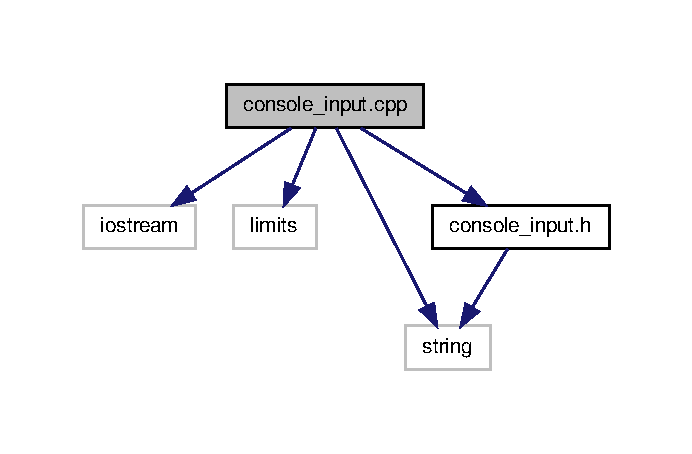
\includegraphics[width=332pt]{console__input_8cpp__incl}
\end{center}
\end{figure}
\subsection*{Functions}
\begin{DoxyCompactItemize}
\item 
double \hyperlink{console__input_8cpp_a8a9df77c5c4adba7ebadb77f3b3dc8ee}{read\-\_\-double} (double min, double max)
\item 
double \hyperlink{console__input_8cpp_a65f2421973540c10e5ae7d10177c566a}{read\-\_\-double} ()
\item 
double \hyperlink{console__input_8cpp_a46878a8594ba71f54911c572031d4614}{read\-\_\-double} (string text)
\item 
double \hyperlink{console__input_8cpp_aca43573be8fe10d4bfede3fc5bd0bd63}{read\-\_\-double} (string text, double min, double max)
\item 
long \hyperlink{console__input_8cpp_a710a686867142de265860584f4147592}{read\-\_\-long} (long min, long max)
\item 
long \hyperlink{console__input_8cpp_a347c616893b725a74f60ea1f7ee325d2}{read\-\_\-long} ()
\item 
long \hyperlink{console__input_8cpp_a9128c63513d87af5259597d8c9930476}{read\-\_\-long} (string text)
\item 
long \hyperlink{console__input_8cpp_a03ebbd2a45117ee03be4e9002210ab36}{read\-\_\-long} (string text, long min, long max)
\item 
int \hyperlink{console__input_8cpp_ad0ccfbb50d0e333ef8acfeab2b7d8071}{read\-\_\-int} (int min, int max)
\item 
int \hyperlink{console__input_8cpp_af310540093ee953c3018bc13bbde3da5}{read\-\_\-int} ()
\item 
int \hyperlink{console__input_8cpp_aaaf3786f6b4803f3120609011de4b0db}{read\-\_\-int} (string text)
\item 
int \hyperlink{console__input_8cpp_a4f8c1bb51d432116d3eda43db3340c8c}{read\-\_\-int} (string text, int min, int max)
\item 
bool \hyperlink{console__input_8cpp_a6bac3909a28fff2736a171022343380b}{read\-\_\-yes\-\_\-no} (string text)
\item 
string \hyperlink{console__input_8cpp_a44ccadd65be527f89bdcf6d27a3b1147}{read\-\_\-text} (string text)
\end{DoxyCompactItemize}


\subsection{Function Documentation}
\hypertarget{console__input_8cpp_a8a9df77c5c4adba7ebadb77f3b3dc8ee}{\index{console\-\_\-input.\-cpp@{console\-\_\-input.\-cpp}!read\-\_\-double@{read\-\_\-double}}
\index{read\-\_\-double@{read\-\_\-double}!console_input.cpp@{console\-\_\-input.\-cpp}}
\subsubsection[{read\-\_\-double}]{\setlength{\rightskip}{0pt plus 5cm}double read\-\_\-double (
\begin{DoxyParamCaption}
\item[{double}]{min, }
\item[{double}]{max}
\end{DoxyParamCaption}
)}}\label{console__input_8cpp_a8a9df77c5c4adba7ebadb77f3b3dc8ee}
Reads a double value in between a given interval from the console. When the entered value is not valid to the interval, the user gets prompted to reenter a valid.


\begin{DoxyParams}{Parameters}
{\em min} & lower bound of the interval. \\
\hline
{\em max} & top bound of the interval\\
\hline
\end{DoxyParams}
\begin{DoxyReturn}{Returns}
a double value in between min and max. 
\end{DoxyReturn}
\hypertarget{console__input_8cpp_a65f2421973540c10e5ae7d10177c566a}{\index{console\-\_\-input.\-cpp@{console\-\_\-input.\-cpp}!read\-\_\-double@{read\-\_\-double}}
\index{read\-\_\-double@{read\-\_\-double}!console_input.cpp@{console\-\_\-input.\-cpp}}
\subsubsection[{read\-\_\-double}]{\setlength{\rightskip}{0pt plus 5cm}double read\-\_\-double (
\begin{DoxyParamCaption}
{}
\end{DoxyParamCaption}
)}}\label{console__input_8cpp_a65f2421973540c10e5ae7d10177c566a}
Reads a double value from the console in between the whole range of double.

\begin{DoxyReturn}{Returns}
a valid double value. 
\end{DoxyReturn}


Here is the call graph for this function\-:\nopagebreak
\begin{figure}[H]
\begin{center}
\leavevmode
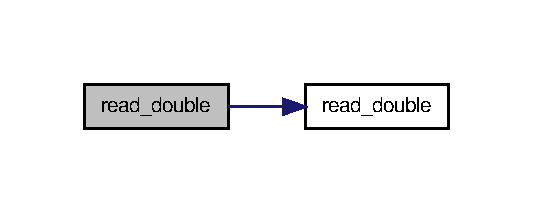
\includegraphics[width=256pt]{console__input_8cpp_a65f2421973540c10e5ae7d10177c566a_cgraph}
\end{center}
\end{figure}


\hypertarget{console__input_8cpp_a46878a8594ba71f54911c572031d4614}{\index{console\-\_\-input.\-cpp@{console\-\_\-input.\-cpp}!read\-\_\-double@{read\-\_\-double}}
\index{read\-\_\-double@{read\-\_\-double}!console_input.cpp@{console\-\_\-input.\-cpp}}
\subsubsection[{read\-\_\-double}]{\setlength{\rightskip}{0pt plus 5cm}double read\-\_\-double (
\begin{DoxyParamCaption}
\item[{string}]{text}
\end{DoxyParamCaption}
)}}\label{console__input_8cpp_a46878a8594ba71f54911c572031d4614}
Prints a text to the console and reads a double value from the console in between the whole range of double.


\begin{DoxyParams}{Parameters}
{\em text} & text to print to the console.\\
\hline
\end{DoxyParams}
\begin{DoxyReturn}{Returns}
a valid double value. 
\end{DoxyReturn}


Here is the call graph for this function\-:\nopagebreak
\begin{figure}[H]
\begin{center}
\leavevmode
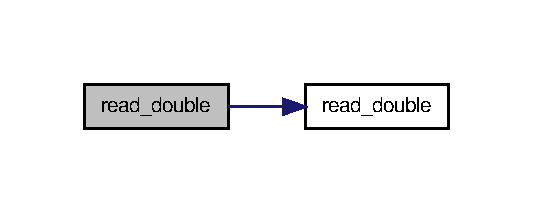
\includegraphics[width=256pt]{console__input_8cpp_a46878a8594ba71f54911c572031d4614_cgraph}
\end{center}
\end{figure}


\hypertarget{console__input_8cpp_aca43573be8fe10d4bfede3fc5bd0bd63}{\index{console\-\_\-input.\-cpp@{console\-\_\-input.\-cpp}!read\-\_\-double@{read\-\_\-double}}
\index{read\-\_\-double@{read\-\_\-double}!console_input.cpp@{console\-\_\-input.\-cpp}}
\subsubsection[{read\-\_\-double}]{\setlength{\rightskip}{0pt plus 5cm}double read\-\_\-double (
\begin{DoxyParamCaption}
\item[{string}]{text, }
\item[{double}]{min, }
\item[{double}]{max}
\end{DoxyParamCaption}
)}}\label{console__input_8cpp_aca43573be8fe10d4bfede3fc5bd0bd63}


Here is the call graph for this function\-:\nopagebreak
\begin{figure}[H]
\begin{center}
\leavevmode
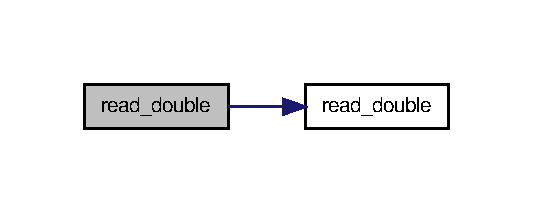
\includegraphics[width=256pt]{console__input_8cpp_aca43573be8fe10d4bfede3fc5bd0bd63_cgraph}
\end{center}
\end{figure}


\hypertarget{console__input_8cpp_ad0ccfbb50d0e333ef8acfeab2b7d8071}{\index{console\-\_\-input.\-cpp@{console\-\_\-input.\-cpp}!read\-\_\-int@{read\-\_\-int}}
\index{read\-\_\-int@{read\-\_\-int}!console_input.cpp@{console\-\_\-input.\-cpp}}
\subsubsection[{read\-\_\-int}]{\setlength{\rightskip}{0pt plus 5cm}int read\-\_\-int (
\begin{DoxyParamCaption}
\item[{int}]{min, }
\item[{int}]{max}
\end{DoxyParamCaption}
)}}\label{console__input_8cpp_ad0ccfbb50d0e333ef8acfeab2b7d8071}
Reads a integer value in between a given interval from the console. When the entered value is not valid to the interval, the user gets prompted to reenter a valid.


\begin{DoxyParams}{Parameters}
{\em min} & lower bound of the interval. \\
\hline
{\em max} & top bound of the interval\\
\hline
\end{DoxyParams}
\begin{DoxyReturn}{Returns}
a int value in between min and max. 
\end{DoxyReturn}


Here is the call graph for this function\-:\nopagebreak
\begin{figure}[H]
\begin{center}
\leavevmode
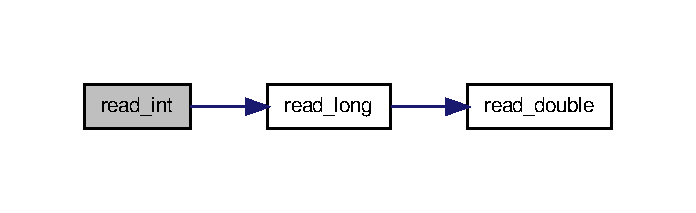
\includegraphics[width=334pt]{console__input_8cpp_ad0ccfbb50d0e333ef8acfeab2b7d8071_cgraph}
\end{center}
\end{figure}


\hypertarget{console__input_8cpp_af310540093ee953c3018bc13bbde3da5}{\index{console\-\_\-input.\-cpp@{console\-\_\-input.\-cpp}!read\-\_\-int@{read\-\_\-int}}
\index{read\-\_\-int@{read\-\_\-int}!console_input.cpp@{console\-\_\-input.\-cpp}}
\subsubsection[{read\-\_\-int}]{\setlength{\rightskip}{0pt plus 5cm}int read\-\_\-int (
\begin{DoxyParamCaption}
{}
\end{DoxyParamCaption}
)}}\label{console__input_8cpp_af310540093ee953c3018bc13bbde3da5}
Reads an integer value from the terminal in between the whole range of long.

\begin{DoxyReturn}{Returns}
a valid integer value. 
\end{DoxyReturn}


Here is the call graph for this function\-:\nopagebreak
\begin{figure}[H]
\begin{center}
\leavevmode
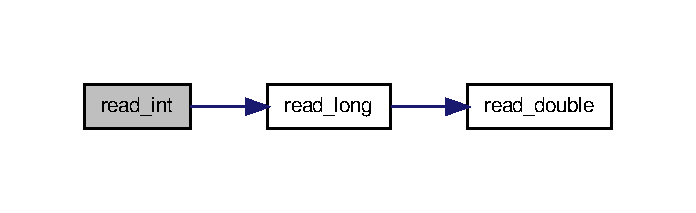
\includegraphics[width=334pt]{console__input_8cpp_af310540093ee953c3018bc13bbde3da5_cgraph}
\end{center}
\end{figure}


\hypertarget{console__input_8cpp_aaaf3786f6b4803f3120609011de4b0db}{\index{console\-\_\-input.\-cpp@{console\-\_\-input.\-cpp}!read\-\_\-int@{read\-\_\-int}}
\index{read\-\_\-int@{read\-\_\-int}!console_input.cpp@{console\-\_\-input.\-cpp}}
\subsubsection[{read\-\_\-int}]{\setlength{\rightskip}{0pt plus 5cm}int read\-\_\-int (
\begin{DoxyParamCaption}
\item[{string}]{text}
\end{DoxyParamCaption}
)}}\label{console__input_8cpp_aaaf3786f6b4803f3120609011de4b0db}
Prints a text to the console and reads a integer value from the console in between the whole range of integer.


\begin{DoxyParams}{Parameters}
{\em text} & text to print to the console.\\
\hline
\end{DoxyParams}
\begin{DoxyReturn}{Returns}
a valid integer value. 
\end{DoxyReturn}


Here is the call graph for this function\-:\nopagebreak
\begin{figure}[H]
\begin{center}
\leavevmode
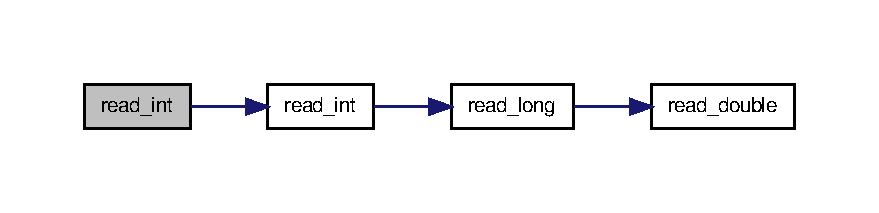
\includegraphics[width=350pt]{console__input_8cpp_aaaf3786f6b4803f3120609011de4b0db_cgraph}
\end{center}
\end{figure}


\hypertarget{console__input_8cpp_a4f8c1bb51d432116d3eda43db3340c8c}{\index{console\-\_\-input.\-cpp@{console\-\_\-input.\-cpp}!read\-\_\-int@{read\-\_\-int}}
\index{read\-\_\-int@{read\-\_\-int}!console_input.cpp@{console\-\_\-input.\-cpp}}
\subsubsection[{read\-\_\-int}]{\setlength{\rightskip}{0pt plus 5cm}int read\-\_\-int (
\begin{DoxyParamCaption}
\item[{string}]{text, }
\item[{int}]{min, }
\item[{int}]{max}
\end{DoxyParamCaption}
)}}\label{console__input_8cpp_a4f8c1bb51d432116d3eda43db3340c8c}
Prints a text to the console and reads a integer value in between a given interval from the console. When the value is not in between the interval, the user gets prompted to reeinter a valid value.


\begin{DoxyParams}{Parameters}
{\em text} & text to print to the console. \\
\hline
{\em min} & lower bound of the interval. \\
\hline
{\em max} & top bound of the interval.\\
\hline
\end{DoxyParams}
\begin{DoxyReturn}{Returns}
a integer value in between min and max. 
\end{DoxyReturn}


Here is the call graph for this function\-:\nopagebreak
\begin{figure}[H]
\begin{center}
\leavevmode
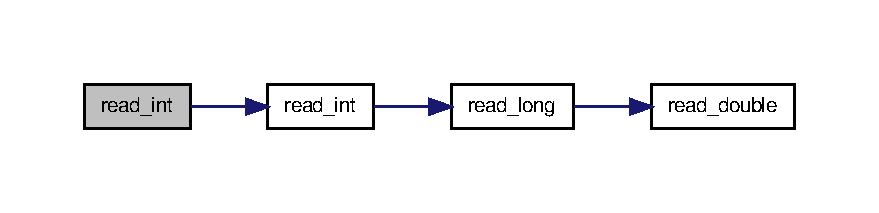
\includegraphics[width=350pt]{console__input_8cpp_a4f8c1bb51d432116d3eda43db3340c8c_cgraph}
\end{center}
\end{figure}


\hypertarget{console__input_8cpp_a710a686867142de265860584f4147592}{\index{console\-\_\-input.\-cpp@{console\-\_\-input.\-cpp}!read\-\_\-long@{read\-\_\-long}}
\index{read\-\_\-long@{read\-\_\-long}!console_input.cpp@{console\-\_\-input.\-cpp}}
\subsubsection[{read\-\_\-long}]{\setlength{\rightskip}{0pt plus 5cm}long read\-\_\-long (
\begin{DoxyParamCaption}
\item[{long}]{min, }
\item[{long}]{max}
\end{DoxyParamCaption}
)}}\label{console__input_8cpp_a710a686867142de265860584f4147592}
Reads a long value in between a given interval from the console. When the entered value is not valid to the interval, the user gets prompted to reenter a valid.


\begin{DoxyParams}{Parameters}
{\em min} & lower bound of the interval. \\
\hline
{\em max} & top bound of the interval\\
\hline
\end{DoxyParams}
\begin{DoxyReturn}{Returns}
a long value in between min and max. 
\end{DoxyReturn}


Here is the call graph for this function\-:\nopagebreak
\begin{figure}[H]
\begin{center}
\leavevmode
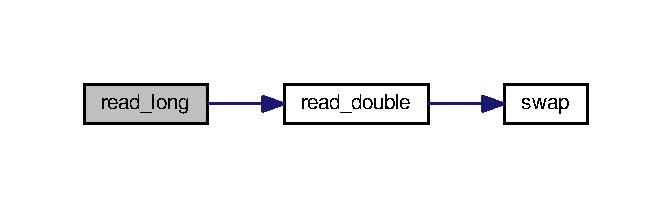
\includegraphics[width=246pt]{console__input_8cpp_a710a686867142de265860584f4147592_cgraph}
\end{center}
\end{figure}


\hypertarget{console__input_8cpp_a347c616893b725a74f60ea1f7ee325d2}{\index{console\-\_\-input.\-cpp@{console\-\_\-input.\-cpp}!read\-\_\-long@{read\-\_\-long}}
\index{read\-\_\-long@{read\-\_\-long}!console_input.cpp@{console\-\_\-input.\-cpp}}
\subsubsection[{read\-\_\-long}]{\setlength{\rightskip}{0pt plus 5cm}long read\-\_\-long (
\begin{DoxyParamCaption}
{}
\end{DoxyParamCaption}
)}}\label{console__input_8cpp_a347c616893b725a74f60ea1f7ee325d2}
Reads a long value from the terminal in between the whole range of long.

\begin{DoxyReturn}{Returns}
a valid long value. 
\end{DoxyReturn}


Here is the call graph for this function\-:\nopagebreak
\begin{figure}[H]
\begin{center}
\leavevmode
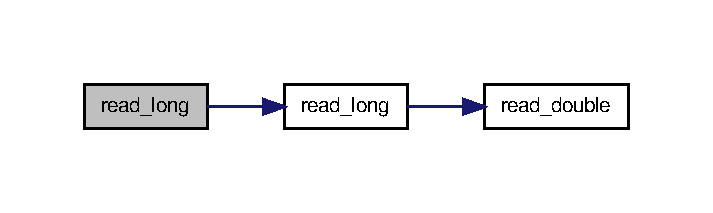
\includegraphics[width=342pt]{console__input_8cpp_a347c616893b725a74f60ea1f7ee325d2_cgraph}
\end{center}
\end{figure}


\hypertarget{console__input_8cpp_a9128c63513d87af5259597d8c9930476}{\index{console\-\_\-input.\-cpp@{console\-\_\-input.\-cpp}!read\-\_\-long@{read\-\_\-long}}
\index{read\-\_\-long@{read\-\_\-long}!console_input.cpp@{console\-\_\-input.\-cpp}}
\subsubsection[{read\-\_\-long}]{\setlength{\rightskip}{0pt plus 5cm}long read\-\_\-long (
\begin{DoxyParamCaption}
\item[{string}]{text}
\end{DoxyParamCaption}
)}}\label{console__input_8cpp_a9128c63513d87af5259597d8c9930476}
Prints a text to the console and reads a long value from the console in between the whole range of long.


\begin{DoxyParams}{Parameters}
{\em text} & text to print to the console.\\
\hline
\end{DoxyParams}
\begin{DoxyReturn}{Returns}
a valid long value. 
\end{DoxyReturn}


Here is the call graph for this function\-:\nopagebreak
\begin{figure}[H]
\begin{center}
\leavevmode
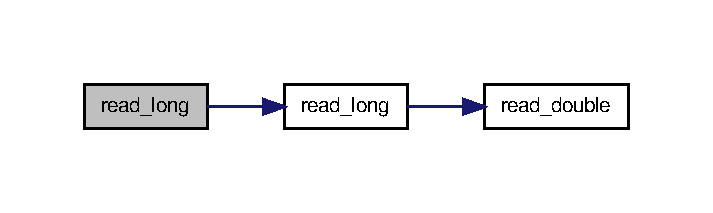
\includegraphics[width=342pt]{console__input_8cpp_a9128c63513d87af5259597d8c9930476_cgraph}
\end{center}
\end{figure}


\hypertarget{console__input_8cpp_a03ebbd2a45117ee03be4e9002210ab36}{\index{console\-\_\-input.\-cpp@{console\-\_\-input.\-cpp}!read\-\_\-long@{read\-\_\-long}}
\index{read\-\_\-long@{read\-\_\-long}!console_input.cpp@{console\-\_\-input.\-cpp}}
\subsubsection[{read\-\_\-long}]{\setlength{\rightskip}{0pt plus 5cm}long read\-\_\-long (
\begin{DoxyParamCaption}
\item[{string}]{text, }
\item[{long}]{min, }
\item[{long}]{max}
\end{DoxyParamCaption}
)}}\label{console__input_8cpp_a03ebbd2a45117ee03be4e9002210ab36}
Prints a text to the console and reads a long value in between a given interval from the console. When the value is not in between the interval, the user gets prompted to reeinter a valid value.


\begin{DoxyParams}{Parameters}
{\em text} & text to print to the console. \\
\hline
{\em min} & lower bound of the interval. \\
\hline
{\em max} & top bound of the interval.\\
\hline
\end{DoxyParams}
\begin{DoxyReturn}{Returns}
a long value in between min and max. 
\end{DoxyReturn}


Here is the call graph for this function\-:\nopagebreak
\begin{figure}[H]
\begin{center}
\leavevmode
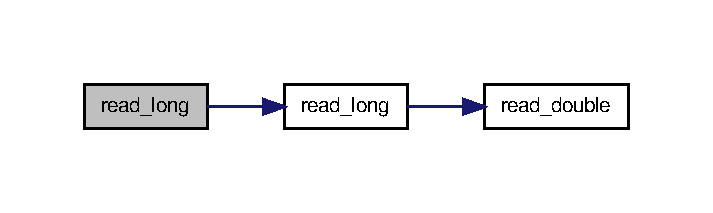
\includegraphics[width=342pt]{console__input_8cpp_a03ebbd2a45117ee03be4e9002210ab36_cgraph}
\end{center}
\end{figure}


\hypertarget{console__input_8cpp_a44ccadd65be527f89bdcf6d27a3b1147}{\index{console\-\_\-input.\-cpp@{console\-\_\-input.\-cpp}!read\-\_\-text@{read\-\_\-text}}
\index{read\-\_\-text@{read\-\_\-text}!console_input.cpp@{console\-\_\-input.\-cpp}}
\subsubsection[{read\-\_\-text}]{\setlength{\rightskip}{0pt plus 5cm}string read\-\_\-text (
\begin{DoxyParamCaption}
\item[{string}]{text}
\end{DoxyParamCaption}
)}}\label{console__input_8cpp_a44ccadd65be527f89bdcf6d27a3b1147}
\hypertarget{console__input_8cpp_a6bac3909a28fff2736a171022343380b}{\index{console\-\_\-input.\-cpp@{console\-\_\-input.\-cpp}!read\-\_\-yes\-\_\-no@{read\-\_\-yes\-\_\-no}}
\index{read\-\_\-yes\-\_\-no@{read\-\_\-yes\-\_\-no}!console_input.cpp@{console\-\_\-input.\-cpp}}
\subsubsection[{read\-\_\-yes\-\_\-no}]{\setlength{\rightskip}{0pt plus 5cm}bool read\-\_\-yes\-\_\-no (
\begin{DoxyParamCaption}
\item[{string}]{text}
\end{DoxyParamCaption}
)}}\label{console__input_8cpp_a6bac3909a28fff2736a171022343380b}

\hypertarget{console__input_8h}{\section{console\-\_\-input.\-h File Reference}
\label{console__input_8h}\index{console\-\_\-input.\-h@{console\-\_\-input.\-h}}
}
{\ttfamily \#include $<$string$>$}\\*
Include dependency graph for console\-\_\-input.\-h\-:\nopagebreak
\begin{figure}[H]
\begin{center}
\leavevmode
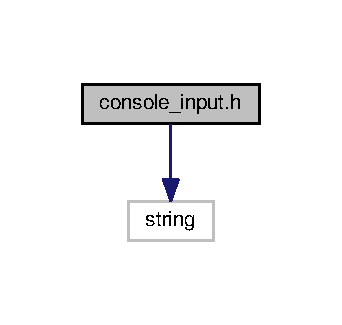
\includegraphics[width=164pt]{console__input_8h__incl}
\end{center}
\end{figure}
This graph shows which files directly or indirectly include this file\-:\nopagebreak
\begin{figure}[H]
\begin{center}
\leavevmode
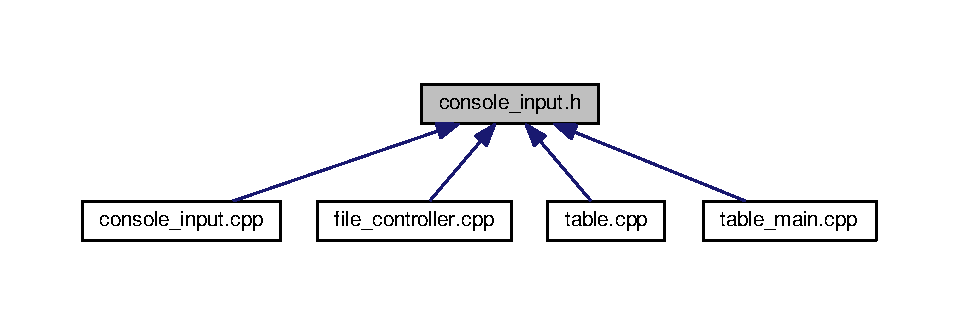
\includegraphics[width=264pt]{console__input_8h__dep__incl}
\end{center}
\end{figure}
\subsection*{Functions}
\begin{DoxyCompactItemize}
\item 
double \hyperlink{console__input_8h_a8a9df77c5c4adba7ebadb77f3b3dc8ee}{read\-\_\-double} (double min, double max)
\item 
double \hyperlink{console__input_8h_a46878a8594ba71f54911c572031d4614}{read\-\_\-double} (string text)
\item 
double \hyperlink{console__input_8h_aca43573be8fe10d4bfede3fc5bd0bd63}{read\-\_\-double} (string text, double min, double max)
\item 
double \hyperlink{console__input_8h_a65f2421973540c10e5ae7d10177c566a}{read\-\_\-double} ()
\item 
void \hyperlink{console__input_8h_afc6e4adf69aec96a5eae4249fbbc7201}{read\-\_\-enter} ()
\item 
long \hyperlink{console__input_8h_a03ebbd2a45117ee03be4e9002210ab36}{read\-\_\-long} (string text, long min, long max)
\item 
long \hyperlink{console__input_8h_a710a686867142de265860584f4147592}{read\-\_\-long} (long min, long max)
\item 
long \hyperlink{console__input_8h_a9128c63513d87af5259597d8c9930476}{read\-\_\-long} (string text)
\item 
long \hyperlink{console__input_8h_a347c616893b725a74f60ea1f7ee325d2}{read\-\_\-long} ()
\item 
int \hyperlink{console__input_8h_a4f8c1bb51d432116d3eda43db3340c8c}{read\-\_\-int} (string text, int min, int max)
\item 
int \hyperlink{console__input_8h_ad0ccfbb50d0e333ef8acfeab2b7d8071}{read\-\_\-int} (int min, int max)
\item 
int \hyperlink{console__input_8h_aaaf3786f6b4803f3120609011de4b0db}{read\-\_\-int} (string text)
\item 
int \hyperlink{console__input_8h_af310540093ee953c3018bc13bbde3da5}{read\-\_\-int} ()
\item 
bool \hyperlink{console__input_8h_a6bac3909a28fff2736a171022343380b}{read\-\_\-yes\-\_\-no} (string text)
\item 
string \hyperlink{console__input_8h_a44ccadd65be527f89bdcf6d27a3b1147}{read\-\_\-text} (string text)
\end{DoxyCompactItemize}


\subsection{Function Documentation}
\hypertarget{console__input_8h_a8a9df77c5c4adba7ebadb77f3b3dc8ee}{\index{console\-\_\-input.\-h@{console\-\_\-input.\-h}!read\-\_\-double@{read\-\_\-double}}
\index{read\-\_\-double@{read\-\_\-double}!console_input.h@{console\-\_\-input.\-h}}
\subsubsection[{read\-\_\-double}]{\setlength{\rightskip}{0pt plus 5cm}double read\-\_\-double (
\begin{DoxyParamCaption}
\item[{double}]{min, }
\item[{double}]{max}
\end{DoxyParamCaption}
)}}\label{console__input_8h_a8a9df77c5c4adba7ebadb77f3b3dc8ee}
Reads a double value in between a given interval from the console. When the entered value is not valid to the interval, the user gets prompted to reenter a valid.


\begin{DoxyParams}{Parameters}
{\em min} & lower bound of the interval. \\
\hline
{\em max} & top bound of the interval\\
\hline
\end{DoxyParams}
\begin{DoxyReturn}{Returns}
a double value in between min and max. 
\end{DoxyReturn}
\hypertarget{console__input_8h_a46878a8594ba71f54911c572031d4614}{\index{console\-\_\-input.\-h@{console\-\_\-input.\-h}!read\-\_\-double@{read\-\_\-double}}
\index{read\-\_\-double@{read\-\_\-double}!console_input.h@{console\-\_\-input.\-h}}
\subsubsection[{read\-\_\-double}]{\setlength{\rightskip}{0pt plus 5cm}double read\-\_\-double (
\begin{DoxyParamCaption}
\item[{string}]{text}
\end{DoxyParamCaption}
)}}\label{console__input_8h_a46878a8594ba71f54911c572031d4614}
Prints a text to the console and reads a double value from the console in between the whole range of double.


\begin{DoxyParams}{Parameters}
{\em text} & text to print to the console.\\
\hline
\end{DoxyParams}
\begin{DoxyReturn}{Returns}
a valid double value. 
\end{DoxyReturn}


Here is the call graph for this function\-:\nopagebreak
\begin{figure}[H]
\begin{center}
\leavevmode
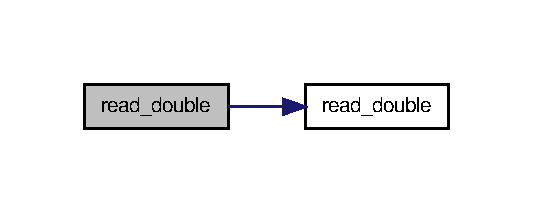
\includegraphics[width=256pt]{console__input_8h_a46878a8594ba71f54911c572031d4614_cgraph}
\end{center}
\end{figure}


\hypertarget{console__input_8h_aca43573be8fe10d4bfede3fc5bd0bd63}{\index{console\-\_\-input.\-h@{console\-\_\-input.\-h}!read\-\_\-double@{read\-\_\-double}}
\index{read\-\_\-double@{read\-\_\-double}!console_input.h@{console\-\_\-input.\-h}}
\subsubsection[{read\-\_\-double}]{\setlength{\rightskip}{0pt plus 5cm}double read\-\_\-double (
\begin{DoxyParamCaption}
\item[{string}]{text, }
\item[{double}]{min, }
\item[{double}]{max}
\end{DoxyParamCaption}
)}}\label{console__input_8h_aca43573be8fe10d4bfede3fc5bd0bd63}


Here is the call graph for this function\-:\nopagebreak
\begin{figure}[H]
\begin{center}
\leavevmode
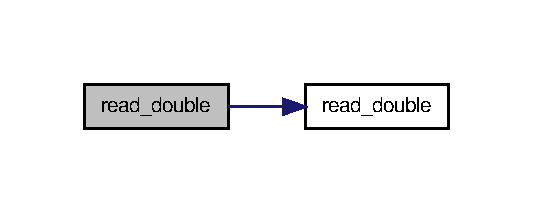
\includegraphics[width=256pt]{console__input_8h_aca43573be8fe10d4bfede3fc5bd0bd63_cgraph}
\end{center}
\end{figure}


\hypertarget{console__input_8h_a65f2421973540c10e5ae7d10177c566a}{\index{console\-\_\-input.\-h@{console\-\_\-input.\-h}!read\-\_\-double@{read\-\_\-double}}
\index{read\-\_\-double@{read\-\_\-double}!console_input.h@{console\-\_\-input.\-h}}
\subsubsection[{read\-\_\-double}]{\setlength{\rightskip}{0pt plus 5cm}double read\-\_\-double (
\begin{DoxyParamCaption}
{}
\end{DoxyParamCaption}
)}}\label{console__input_8h_a65f2421973540c10e5ae7d10177c566a}
Reads a double value from the console in between the whole range of double.

\begin{DoxyReturn}{Returns}
a valid double value. 
\end{DoxyReturn}


Here is the call graph for this function\-:\nopagebreak
\begin{figure}[H]
\begin{center}
\leavevmode
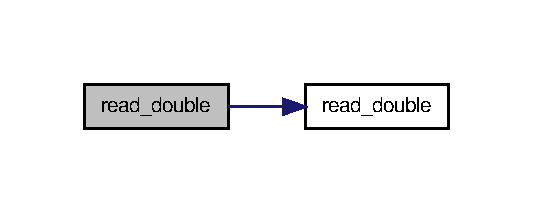
\includegraphics[width=256pt]{console__input_8h_a65f2421973540c10e5ae7d10177c566a_cgraph}
\end{center}
\end{figure}


\hypertarget{console__input_8h_afc6e4adf69aec96a5eae4249fbbc7201}{\index{console\-\_\-input.\-h@{console\-\_\-input.\-h}!read\-\_\-enter@{read\-\_\-enter}}
\index{read\-\_\-enter@{read\-\_\-enter}!console_input.h@{console\-\_\-input.\-h}}
\subsubsection[{read\-\_\-enter}]{\setlength{\rightskip}{0pt plus 5cm}void read\-\_\-enter (
\begin{DoxyParamCaption}
{}
\end{DoxyParamCaption}
)}}\label{console__input_8h_afc6e4adf69aec96a5eae4249fbbc7201}
\hypertarget{console__input_8h_a4f8c1bb51d432116d3eda43db3340c8c}{\index{console\-\_\-input.\-h@{console\-\_\-input.\-h}!read\-\_\-int@{read\-\_\-int}}
\index{read\-\_\-int@{read\-\_\-int}!console_input.h@{console\-\_\-input.\-h}}
\subsubsection[{read\-\_\-int}]{\setlength{\rightskip}{0pt plus 5cm}int read\-\_\-int (
\begin{DoxyParamCaption}
\item[{string}]{text, }
\item[{int}]{min, }
\item[{int}]{max}
\end{DoxyParamCaption}
)}}\label{console__input_8h_a4f8c1bb51d432116d3eda43db3340c8c}
Prints a text to the console and reads a integer value in between a given interval from the console. When the value is not in between the interval, the user gets prompted to reeinter a valid value.


\begin{DoxyParams}{Parameters}
{\em text} & text to print to the console. \\
\hline
{\em min} & lower bound of the interval. \\
\hline
{\em max} & top bound of the interval.\\
\hline
\end{DoxyParams}
\begin{DoxyReturn}{Returns}
a integer value in between min and max. 
\end{DoxyReturn}


Here is the call graph for this function\-:\nopagebreak
\begin{figure}[H]
\begin{center}
\leavevmode
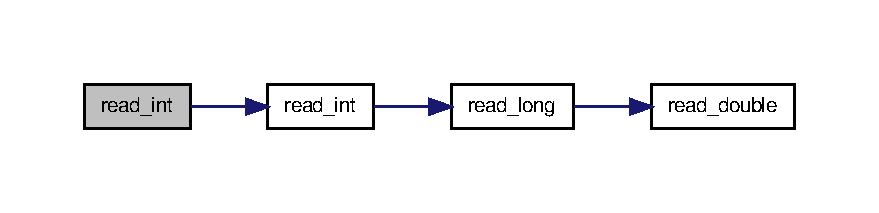
\includegraphics[width=350pt]{console__input_8h_a4f8c1bb51d432116d3eda43db3340c8c_cgraph}
\end{center}
\end{figure}


\hypertarget{console__input_8h_ad0ccfbb50d0e333ef8acfeab2b7d8071}{\index{console\-\_\-input.\-h@{console\-\_\-input.\-h}!read\-\_\-int@{read\-\_\-int}}
\index{read\-\_\-int@{read\-\_\-int}!console_input.h@{console\-\_\-input.\-h}}
\subsubsection[{read\-\_\-int}]{\setlength{\rightskip}{0pt plus 5cm}int read\-\_\-int (
\begin{DoxyParamCaption}
\item[{int}]{min, }
\item[{int}]{max}
\end{DoxyParamCaption}
)}}\label{console__input_8h_ad0ccfbb50d0e333ef8acfeab2b7d8071}
Reads a integer value in between a given interval from the console. When the entered value is not valid to the interval, the user gets prompted to reenter a valid.


\begin{DoxyParams}{Parameters}
{\em min} & lower bound of the interval. \\
\hline
{\em max} & top bound of the interval\\
\hline
\end{DoxyParams}
\begin{DoxyReturn}{Returns}
a int value in between min and max. 
\end{DoxyReturn}


Here is the call graph for this function\-:\nopagebreak
\begin{figure}[H]
\begin{center}
\leavevmode
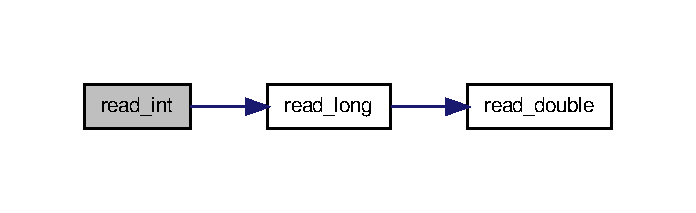
\includegraphics[width=334pt]{console__input_8h_ad0ccfbb50d0e333ef8acfeab2b7d8071_cgraph}
\end{center}
\end{figure}


\hypertarget{console__input_8h_aaaf3786f6b4803f3120609011de4b0db}{\index{console\-\_\-input.\-h@{console\-\_\-input.\-h}!read\-\_\-int@{read\-\_\-int}}
\index{read\-\_\-int@{read\-\_\-int}!console_input.h@{console\-\_\-input.\-h}}
\subsubsection[{read\-\_\-int}]{\setlength{\rightskip}{0pt plus 5cm}int read\-\_\-int (
\begin{DoxyParamCaption}
\item[{string}]{text}
\end{DoxyParamCaption}
)}}\label{console__input_8h_aaaf3786f6b4803f3120609011de4b0db}
Prints a text to the console and reads a integer value from the console in between the whole range of integer.


\begin{DoxyParams}{Parameters}
{\em text} & text to print to the console.\\
\hline
\end{DoxyParams}
\begin{DoxyReturn}{Returns}
a valid integer value. 
\end{DoxyReturn}


Here is the call graph for this function\-:\nopagebreak
\begin{figure}[H]
\begin{center}
\leavevmode
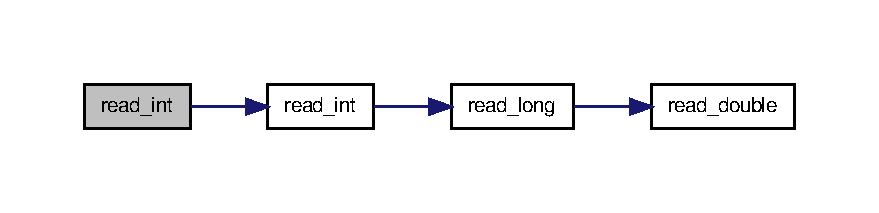
\includegraphics[width=350pt]{console__input_8h_aaaf3786f6b4803f3120609011de4b0db_cgraph}
\end{center}
\end{figure}


\hypertarget{console__input_8h_af310540093ee953c3018bc13bbde3da5}{\index{console\-\_\-input.\-h@{console\-\_\-input.\-h}!read\-\_\-int@{read\-\_\-int}}
\index{read\-\_\-int@{read\-\_\-int}!console_input.h@{console\-\_\-input.\-h}}
\subsubsection[{read\-\_\-int}]{\setlength{\rightskip}{0pt plus 5cm}int read\-\_\-int (
\begin{DoxyParamCaption}
{}
\end{DoxyParamCaption}
)}}\label{console__input_8h_af310540093ee953c3018bc13bbde3da5}
Reads an integer value from the terminal in between the whole range of long.

\begin{DoxyReturn}{Returns}
a valid integer value. 
\end{DoxyReturn}


Here is the call graph for this function\-:\nopagebreak
\begin{figure}[H]
\begin{center}
\leavevmode
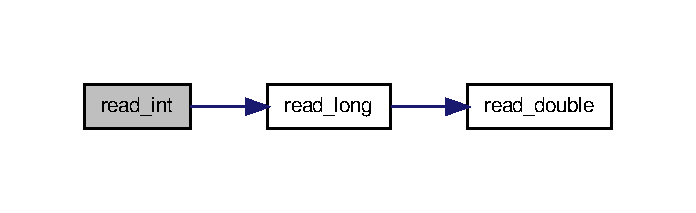
\includegraphics[width=334pt]{console__input_8h_af310540093ee953c3018bc13bbde3da5_cgraph}
\end{center}
\end{figure}


\hypertarget{console__input_8h_a03ebbd2a45117ee03be4e9002210ab36}{\index{console\-\_\-input.\-h@{console\-\_\-input.\-h}!read\-\_\-long@{read\-\_\-long}}
\index{read\-\_\-long@{read\-\_\-long}!console_input.h@{console\-\_\-input.\-h}}
\subsubsection[{read\-\_\-long}]{\setlength{\rightskip}{0pt plus 5cm}long read\-\_\-long (
\begin{DoxyParamCaption}
\item[{string}]{text, }
\item[{long}]{min, }
\item[{long}]{max}
\end{DoxyParamCaption}
)}}\label{console__input_8h_a03ebbd2a45117ee03be4e9002210ab36}
Prints a text to the console and reads a long value in between a given interval from the console. When the value is not in between the interval, the user gets prompted to reeinter a valid value.


\begin{DoxyParams}{Parameters}
{\em text} & text to print to the console. \\
\hline
{\em min} & lower bound of the interval. \\
\hline
{\em max} & top bound of the interval.\\
\hline
\end{DoxyParams}
\begin{DoxyReturn}{Returns}
a long value in between min and max. 
\end{DoxyReturn}


Here is the call graph for this function\-:\nopagebreak
\begin{figure}[H]
\begin{center}
\leavevmode
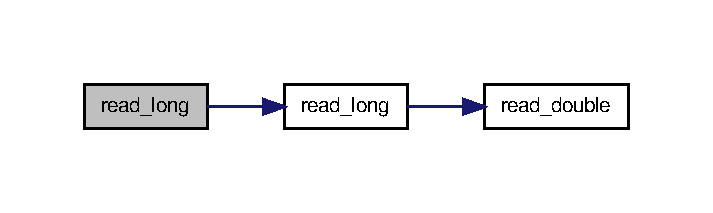
\includegraphics[width=342pt]{console__input_8h_a03ebbd2a45117ee03be4e9002210ab36_cgraph}
\end{center}
\end{figure}


\hypertarget{console__input_8h_a710a686867142de265860584f4147592}{\index{console\-\_\-input.\-h@{console\-\_\-input.\-h}!read\-\_\-long@{read\-\_\-long}}
\index{read\-\_\-long@{read\-\_\-long}!console_input.h@{console\-\_\-input.\-h}}
\subsubsection[{read\-\_\-long}]{\setlength{\rightskip}{0pt plus 5cm}long read\-\_\-long (
\begin{DoxyParamCaption}
\item[{long}]{min, }
\item[{long}]{max}
\end{DoxyParamCaption}
)}}\label{console__input_8h_a710a686867142de265860584f4147592}
Reads a long value in between a given interval from the console. When the entered value is not valid to the interval, the user gets prompted to reenter a valid.


\begin{DoxyParams}{Parameters}
{\em min} & lower bound of the interval. \\
\hline
{\em max} & top bound of the interval\\
\hline
\end{DoxyParams}
\begin{DoxyReturn}{Returns}
a long value in between min and max. 
\end{DoxyReturn}


Here is the call graph for this function\-:\nopagebreak
\begin{figure}[H]
\begin{center}
\leavevmode
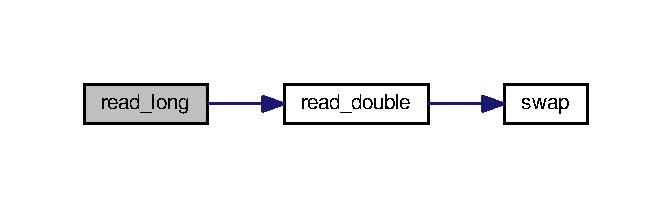
\includegraphics[width=246pt]{console__input_8h_a710a686867142de265860584f4147592_cgraph}
\end{center}
\end{figure}


\hypertarget{console__input_8h_a9128c63513d87af5259597d8c9930476}{\index{console\-\_\-input.\-h@{console\-\_\-input.\-h}!read\-\_\-long@{read\-\_\-long}}
\index{read\-\_\-long@{read\-\_\-long}!console_input.h@{console\-\_\-input.\-h}}
\subsubsection[{read\-\_\-long}]{\setlength{\rightskip}{0pt plus 5cm}long read\-\_\-long (
\begin{DoxyParamCaption}
\item[{string}]{text}
\end{DoxyParamCaption}
)}}\label{console__input_8h_a9128c63513d87af5259597d8c9930476}
Prints a text to the console and reads a long value from the console in between the whole range of long.


\begin{DoxyParams}{Parameters}
{\em text} & text to print to the console.\\
\hline
\end{DoxyParams}
\begin{DoxyReturn}{Returns}
a valid long value. 
\end{DoxyReturn}


Here is the call graph for this function\-:\nopagebreak
\begin{figure}[H]
\begin{center}
\leavevmode
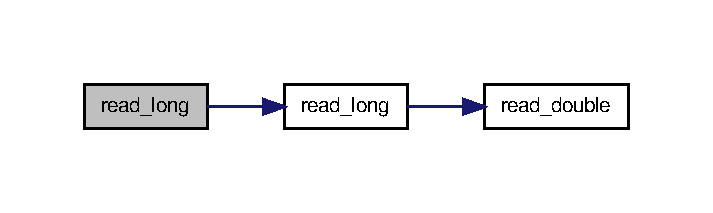
\includegraphics[width=342pt]{console__input_8h_a9128c63513d87af5259597d8c9930476_cgraph}
\end{center}
\end{figure}


\hypertarget{console__input_8h_a347c616893b725a74f60ea1f7ee325d2}{\index{console\-\_\-input.\-h@{console\-\_\-input.\-h}!read\-\_\-long@{read\-\_\-long}}
\index{read\-\_\-long@{read\-\_\-long}!console_input.h@{console\-\_\-input.\-h}}
\subsubsection[{read\-\_\-long}]{\setlength{\rightskip}{0pt plus 5cm}long read\-\_\-long (
\begin{DoxyParamCaption}
{}
\end{DoxyParamCaption}
)}}\label{console__input_8h_a347c616893b725a74f60ea1f7ee325d2}
Reads a long value from the terminal in between the whole range of long.

\begin{DoxyReturn}{Returns}
a valid long value. 
\end{DoxyReturn}


Here is the call graph for this function\-:\nopagebreak
\begin{figure}[H]
\begin{center}
\leavevmode
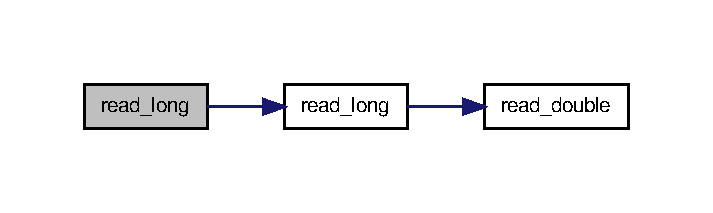
\includegraphics[width=342pt]{console__input_8h_a347c616893b725a74f60ea1f7ee325d2_cgraph}
\end{center}
\end{figure}


\hypertarget{console__input_8h_a44ccadd65be527f89bdcf6d27a3b1147}{\index{console\-\_\-input.\-h@{console\-\_\-input.\-h}!read\-\_\-text@{read\-\_\-text}}
\index{read\-\_\-text@{read\-\_\-text}!console_input.h@{console\-\_\-input.\-h}}
\subsubsection[{read\-\_\-text}]{\setlength{\rightskip}{0pt plus 5cm}string read\-\_\-text (
\begin{DoxyParamCaption}
\item[{string}]{text}
\end{DoxyParamCaption}
)}}\label{console__input_8h_a44ccadd65be527f89bdcf6d27a3b1147}
\hypertarget{console__input_8h_a6bac3909a28fff2736a171022343380b}{\index{console\-\_\-input.\-h@{console\-\_\-input.\-h}!read\-\_\-yes\-\_\-no@{read\-\_\-yes\-\_\-no}}
\index{read\-\_\-yes\-\_\-no@{read\-\_\-yes\-\_\-no}!console_input.h@{console\-\_\-input.\-h}}
\subsubsection[{read\-\_\-yes\-\_\-no}]{\setlength{\rightskip}{0pt plus 5cm}bool read\-\_\-yes\-\_\-no (
\begin{DoxyParamCaption}
\item[{string}]{text}
\end{DoxyParamCaption}
)}}\label{console__input_8h_a6bac3909a28fff2736a171022343380b}

\hypertarget{file__controller_8cpp}{\section{file\-\_\-controller.\-cpp File Reference}
\label{file__controller_8cpp}\index{file\-\_\-controller.\-cpp@{file\-\_\-controller.\-cpp}}
}
{\ttfamily \#include $<$iostream$>$}\\*
{\ttfamily \#include $<$string$>$}\\*
{\ttfamily \#include $<$fstream$>$}\\*
{\ttfamily \#include \char`\"{}console\-\_\-input.\-h\char`\"{}}\\*
{\ttfamily \#include \char`\"{}file\-\_\-controller.\-h\char`\"{}}\\*
Include dependency graph for file\-\_\-controller.\-cpp\-:\nopagebreak
\begin{figure}[H]
\begin{center}
\leavevmode
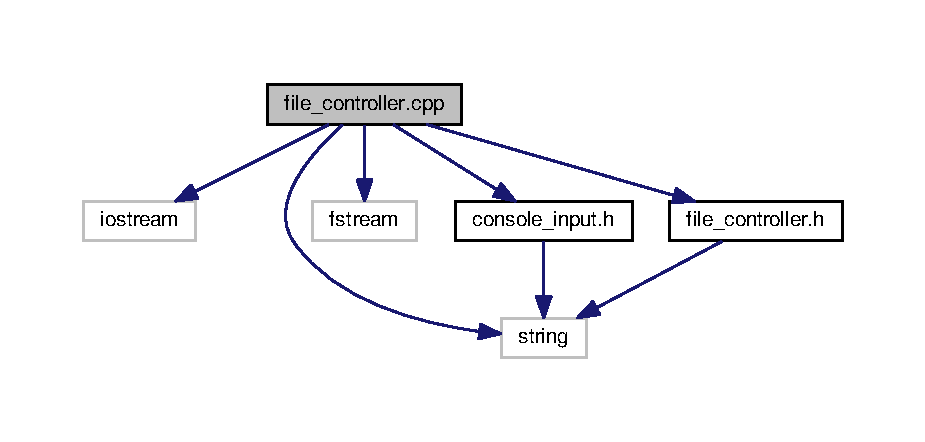
\includegraphics[width=350pt]{file__controller_8cpp__incl}
\end{center}
\end{figure}
\subsection*{Functions}
\begin{DoxyCompactItemize}
\item 
void \hyperlink{file__controller_8cpp_a8600a74cc7b9657c803885b9f6844fe7}{write\-\_\-to\-\_\-file} (string filename, string text, bool secure)
\item 
void \hyperlink{file__controller_8cpp_a90ee1f4929750a48a0e201f8923a2449}{write\-\_\-to\-\_\-file} (string text)
\item 
bool \hyperlink{file__controller_8cpp_acde73c899ec0618eeb8ae54b0a823f39}{file\-\_\-exists} (const std\-::string \&filename)
\item 
string \hyperlink{file__controller_8cpp_a5b269a712c2a290dd75694ab5ed3cb18}{read\-\_\-secure\-\_\-filename} ()
\end{DoxyCompactItemize}


\subsection{Function Documentation}
\hypertarget{file__controller_8cpp_acde73c899ec0618eeb8ae54b0a823f39}{\index{file\-\_\-controller.\-cpp@{file\-\_\-controller.\-cpp}!file\-\_\-exists@{file\-\_\-exists}}
\index{file\-\_\-exists@{file\-\_\-exists}!file_controller.cpp@{file\-\_\-controller.\-cpp}}
\subsubsection[{file\-\_\-exists}]{\setlength{\rightskip}{0pt plus 5cm}bool file\-\_\-exists (
\begin{DoxyParamCaption}
\item[{const std\-::string \&}]{filename}
\end{DoxyParamCaption}
)}}\label{file__controller_8cpp_acde73c899ec0618eeb8ae54b0a823f39}
Checks if a file already exists by its name.


\begin{DoxyParams}{Parameters}
{\em filename} & Filename to check for existence.\\
\hline
\end{DoxyParams}
\begin{DoxyReturn}{Returns}
true when the file exists. false when the file don't exists. 
\end{DoxyReturn}
\hypertarget{file__controller_8cpp_a5b269a712c2a290dd75694ab5ed3cb18}{\index{file\-\_\-controller.\-cpp@{file\-\_\-controller.\-cpp}!read\-\_\-secure\-\_\-filename@{read\-\_\-secure\-\_\-filename}}
\index{read\-\_\-secure\-\_\-filename@{read\-\_\-secure\-\_\-filename}!file_controller.cpp@{file\-\_\-controller.\-cpp}}
\subsubsection[{read\-\_\-secure\-\_\-filename}]{\setlength{\rightskip}{0pt plus 5cm}string read\-\_\-secure\-\_\-filename (
\begin{DoxyParamCaption}
{}
\end{DoxyParamCaption}
)}}\label{file__controller_8cpp_a5b269a712c2a290dd75694ab5ed3cb18}
Promts the user to enter a filename. The filename gets checked for existance. When there is already an existing file for the enterd filename, the user gets promted to override or reenter e new name.

\begin{DoxyReturn}{Returns}
a filename of a new file or of an existing file which can be overwritten. 
\end{DoxyReturn}


Here is the call graph for this function\-:\nopagebreak
\begin{figure}[H]
\begin{center}
\leavevmode
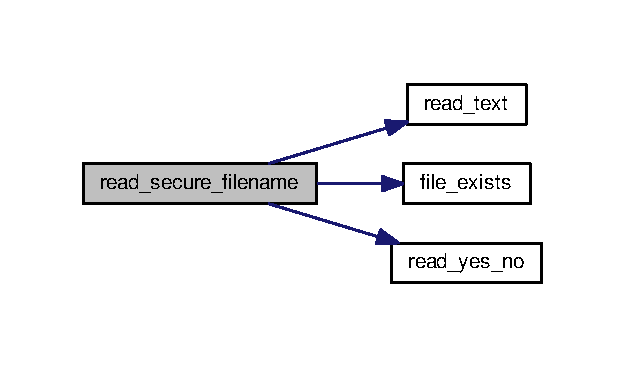
\includegraphics[width=300pt]{file__controller_8cpp_a5b269a712c2a290dd75694ab5ed3cb18_cgraph}
\end{center}
\end{figure}


\hypertarget{file__controller_8cpp_a8600a74cc7b9657c803885b9f6844fe7}{\index{file\-\_\-controller.\-cpp@{file\-\_\-controller.\-cpp}!write\-\_\-to\-\_\-file@{write\-\_\-to\-\_\-file}}
\index{write\-\_\-to\-\_\-file@{write\-\_\-to\-\_\-file}!file_controller.cpp@{file\-\_\-controller.\-cpp}}
\subsubsection[{write\-\_\-to\-\_\-file}]{\setlength{\rightskip}{0pt plus 5cm}void write\-\_\-to\-\_\-file (
\begin{DoxyParamCaption}
\item[{string}]{filename, }
\item[{string}]{text, }
\item[{bool}]{secure}
\end{DoxyParamCaption}
)}}\label{file__controller_8cpp_a8600a74cc7b9657c803885b9f6844fe7}
Writes given text into a file with the given filename.


\begin{DoxyParams}{Parameters}
{\em filename} & Name of the file to wirte. \\
\hline
{\em text} & Text to write into the file. \\
\hline
\end{DoxyParams}


Here is the call graph for this function\-:\nopagebreak
\begin{figure}[H]
\begin{center}
\leavevmode
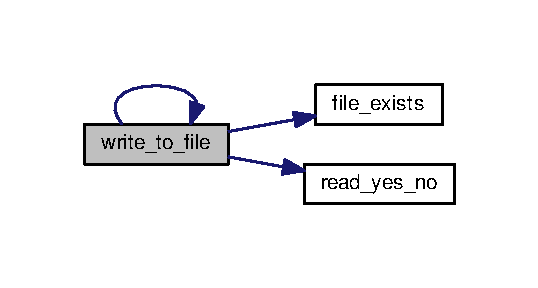
\includegraphics[width=258pt]{file__controller_8cpp_a8600a74cc7b9657c803885b9f6844fe7_cgraph}
\end{center}
\end{figure}


\hypertarget{file__controller_8cpp_a90ee1f4929750a48a0e201f8923a2449}{\index{file\-\_\-controller.\-cpp@{file\-\_\-controller.\-cpp}!write\-\_\-to\-\_\-file@{write\-\_\-to\-\_\-file}}
\index{write\-\_\-to\-\_\-file@{write\-\_\-to\-\_\-file}!file_controller.cpp@{file\-\_\-controller.\-cpp}}
\subsubsection[{write\-\_\-to\-\_\-file}]{\setlength{\rightskip}{0pt plus 5cm}void write\-\_\-to\-\_\-file (
\begin{DoxyParamCaption}
\item[{string}]{text}
\end{DoxyParamCaption}
)}}\label{file__controller_8cpp_a90ee1f4929750a48a0e201f8923a2449}
Writes a given text into a file. The name of the file has to be entered by the user. When the file already exists. The user gets prompted to overwrite or entering a new name.


\begin{DoxyParams}{Parameters}
{\em text} & Text to write into the file. \\
\hline
\end{DoxyParams}


Here is the call graph for this function\-:\nopagebreak
\begin{figure}[H]
\begin{center}
\leavevmode
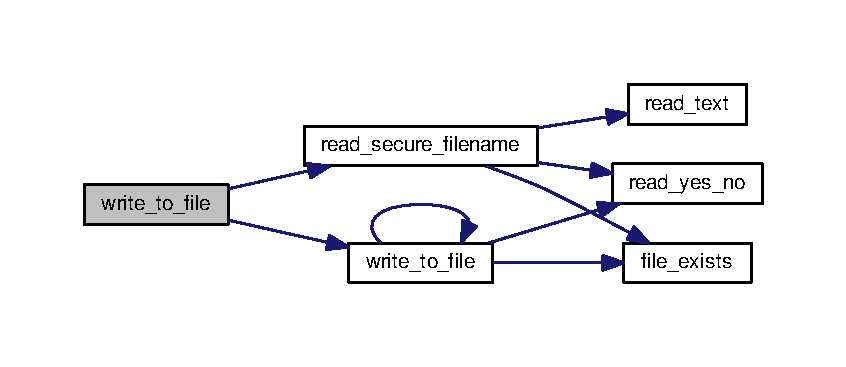
\includegraphics[width=350pt]{file__controller_8cpp_a90ee1f4929750a48a0e201f8923a2449_cgraph}
\end{center}
\end{figure}



\hypertarget{file__controller_8h}{\section{file\-\_\-controller.\-h File Reference}
\label{file__controller_8h}\index{file\-\_\-controller.\-h@{file\-\_\-controller.\-h}}
}
{\ttfamily \#include $<$string$>$}\\*
Include dependency graph for file\-\_\-controller.\-h\-:\nopagebreak
\begin{figure}[H]
\begin{center}
\leavevmode
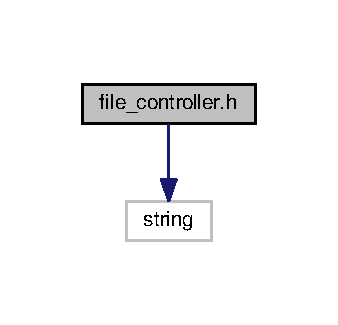
\includegraphics[width=162pt]{file__controller_8h__incl}
\end{center}
\end{figure}
This graph shows which files directly or indirectly include this file\-:\nopagebreak
\begin{figure}[H]
\begin{center}
\leavevmode
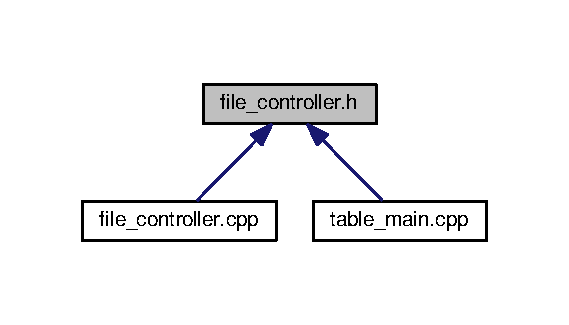
\includegraphics[width=273pt]{file__controller_8h__dep__incl}
\end{center}
\end{figure}
\subsection*{Functions}
\begin{DoxyCompactItemize}
\item 
void \hyperlink{file__controller_8h_aff23a80c6148171c9745ed0c31704e83}{write\-\_\-to\-\_\-file} (string filename, string text, bool secure=true)
\item 
void \hyperlink{file__controller_8h_a90ee1f4929750a48a0e201f8923a2449}{write\-\_\-to\-\_\-file} (string text)
\item 
bool \hyperlink{file__controller_8h_acde73c899ec0618eeb8ae54b0a823f39}{file\-\_\-exists} (const std\-::string \&filename)
\item 
string \hyperlink{file__controller_8h_a5b269a712c2a290dd75694ab5ed3cb18}{read\-\_\-secure\-\_\-filename} ()
\item 
void \hyperlink{file__controller_8h_a8dace9e9ce4bc664cfa4862a21a70c25}{show\-\_\-file} (string filename)
\end{DoxyCompactItemize}


\subsection{Function Documentation}
\hypertarget{file__controller_8h_acde73c899ec0618eeb8ae54b0a823f39}{\index{file\-\_\-controller.\-h@{file\-\_\-controller.\-h}!file\-\_\-exists@{file\-\_\-exists}}
\index{file\-\_\-exists@{file\-\_\-exists}!file_controller.h@{file\-\_\-controller.\-h}}
\subsubsection[{file\-\_\-exists}]{\setlength{\rightskip}{0pt plus 5cm}bool file\-\_\-exists (
\begin{DoxyParamCaption}
\item[{const std\-::string \&}]{filename}
\end{DoxyParamCaption}
)}}\label{file__controller_8h_acde73c899ec0618eeb8ae54b0a823f39}
Checks if a file already exists by its name.


\begin{DoxyParams}{Parameters}
{\em filename} & Filename to check for existence.\\
\hline
\end{DoxyParams}
\begin{DoxyReturn}{Returns}
true when the file exists. false when the file don't exists. 
\end{DoxyReturn}
\hypertarget{file__controller_8h_a5b269a712c2a290dd75694ab5ed3cb18}{\index{file\-\_\-controller.\-h@{file\-\_\-controller.\-h}!read\-\_\-secure\-\_\-filename@{read\-\_\-secure\-\_\-filename}}
\index{read\-\_\-secure\-\_\-filename@{read\-\_\-secure\-\_\-filename}!file_controller.h@{file\-\_\-controller.\-h}}
\subsubsection[{read\-\_\-secure\-\_\-filename}]{\setlength{\rightskip}{0pt plus 5cm}string read\-\_\-secure\-\_\-filename (
\begin{DoxyParamCaption}
{}
\end{DoxyParamCaption}
)}}\label{file__controller_8h_a5b269a712c2a290dd75694ab5ed3cb18}
Promts the user to enter a filename. The filename gets checked for existance. When there is already an existing file for the enterd filename, the user gets promted to override or reenter e new name.

\begin{DoxyReturn}{Returns}
a filename of a new file or of an existing file which can be overwritten. 
\end{DoxyReturn}


Here is the call graph for this function\-:\nopagebreak
\begin{figure}[H]
\begin{center}
\leavevmode
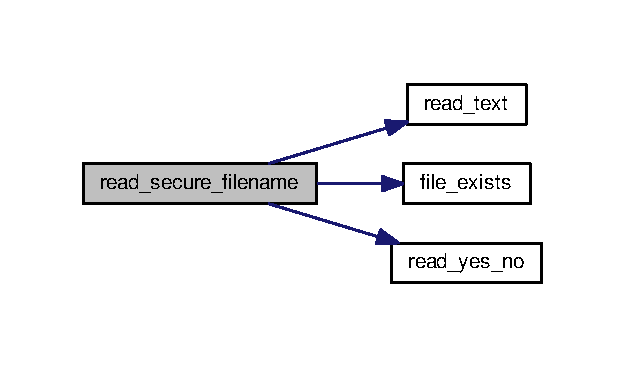
\includegraphics[width=300pt]{file__controller_8h_a5b269a712c2a290dd75694ab5ed3cb18_cgraph}
\end{center}
\end{figure}


\hypertarget{file__controller_8h_a8dace9e9ce4bc664cfa4862a21a70c25}{\index{file\-\_\-controller.\-h@{file\-\_\-controller.\-h}!show\-\_\-file@{show\-\_\-file}}
\index{show\-\_\-file@{show\-\_\-file}!file_controller.h@{file\-\_\-controller.\-h}}
\subsubsection[{show\-\_\-file}]{\setlength{\rightskip}{0pt plus 5cm}void show\-\_\-file (
\begin{DoxyParamCaption}
\item[{string}]{filename}
\end{DoxyParamCaption}
)}}\label{file__controller_8h_a8dace9e9ce4bc664cfa4862a21a70c25}
Reads a file according a given filename and prints the content to the console.


\begin{DoxyParams}{Parameters}
{\em filename} & Name of the file to print to the console. \\
\hline
\end{DoxyParams}
\hypertarget{file__controller_8h_aff23a80c6148171c9745ed0c31704e83}{\index{file\-\_\-controller.\-h@{file\-\_\-controller.\-h}!write\-\_\-to\-\_\-file@{write\-\_\-to\-\_\-file}}
\index{write\-\_\-to\-\_\-file@{write\-\_\-to\-\_\-file}!file_controller.h@{file\-\_\-controller.\-h}}
\subsubsection[{write\-\_\-to\-\_\-file}]{\setlength{\rightskip}{0pt plus 5cm}void write\-\_\-to\-\_\-file (
\begin{DoxyParamCaption}
\item[{string}]{filename, }
\item[{string}]{text, }
\item[{bool}]{secure}
\end{DoxyParamCaption}
)}}\label{file__controller_8h_aff23a80c6148171c9745ed0c31704e83}
Writes given text into a file with the given filename.


\begin{DoxyParams}{Parameters}
{\em filename} & Name of the file to wirte. \\
\hline
{\em text} & Text to write into the file. \\
\hline
\end{DoxyParams}


Here is the call graph for this function\-:\nopagebreak
\begin{figure}[H]
\begin{center}
\leavevmode
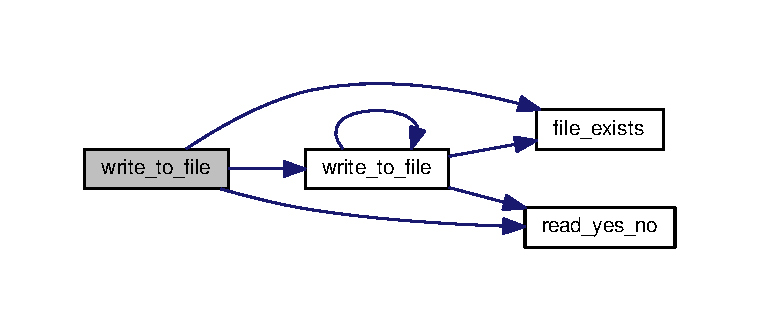
\includegraphics[width=350pt]{file__controller_8h_aff23a80c6148171c9745ed0c31704e83_cgraph}
\end{center}
\end{figure}


\hypertarget{file__controller_8h_a90ee1f4929750a48a0e201f8923a2449}{\index{file\-\_\-controller.\-h@{file\-\_\-controller.\-h}!write\-\_\-to\-\_\-file@{write\-\_\-to\-\_\-file}}
\index{write\-\_\-to\-\_\-file@{write\-\_\-to\-\_\-file}!file_controller.h@{file\-\_\-controller.\-h}}
\subsubsection[{write\-\_\-to\-\_\-file}]{\setlength{\rightskip}{0pt plus 5cm}void write\-\_\-to\-\_\-file (
\begin{DoxyParamCaption}
\item[{string}]{text}
\end{DoxyParamCaption}
)}}\label{file__controller_8h_a90ee1f4929750a48a0e201f8923a2449}
Writes a given text into a file. The name of the file has to be entered by the user. When the file already exists. The user gets prompted to overwrite or entering a new name.


\begin{DoxyParams}{Parameters}
{\em text} & Text to write into the file. \\
\hline
\end{DoxyParams}


Here is the call graph for this function\-:\nopagebreak
\begin{figure}[H]
\begin{center}
\leavevmode
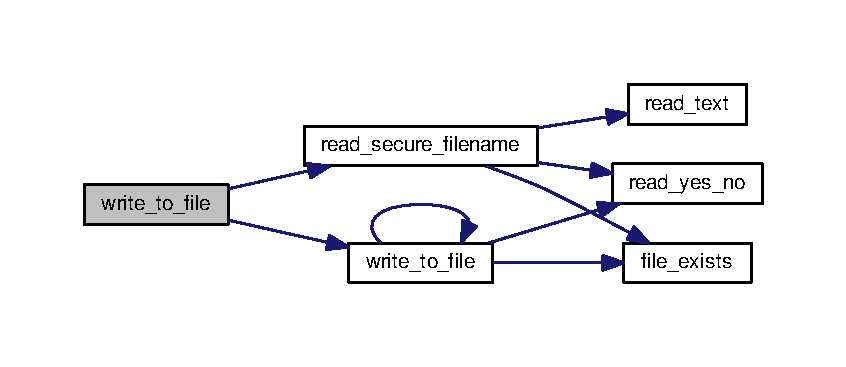
\includegraphics[width=350pt]{file__controller_8h_a90ee1f4929750a48a0e201f8923a2449_cgraph}
\end{center}
\end{figure}



\hypertarget{io__util_8cpp}{\section{io\-\_\-util.\-cpp File Reference}
\label{io__util_8cpp}\index{io\-\_\-util.\-cpp@{io\-\_\-util.\-cpp}}
}
{\ttfamily \#include $<$iostream$>$}\\*
Include dependency graph for io\-\_\-util.\-cpp\-:
\nopagebreak
\begin{figure}[H]
\begin{center}
\leavevmode
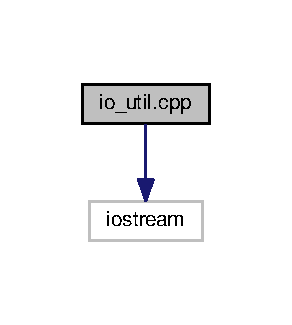
\includegraphics[width=140pt]{io__util_8cpp__incl}
\end{center}
\end{figure}
\subsection*{Functions}
\begin{DoxyCompactItemize}
\item 
void \hyperlink{io__util_8cpp_ae8c346aa92fc891022a940f2c5c75f95}{setze\-\_\-schalter} (ios\-\_\-base\-::fmtflags format)
\item 
void \hyperlink{io__util_8cpp_acd3415eef442ced2b5e064f95f04b624}{swap} (int $\ast$x, int $\ast$y)
\end{DoxyCompactItemize}


\subsection{Function Documentation}
\hypertarget{io__util_8cpp_ae8c346aa92fc891022a940f2c5c75f95}{\index{io\-\_\-util.\-cpp@{io\-\_\-util.\-cpp}!setze\-\_\-schalter@{setze\-\_\-schalter}}
\index{setze\-\_\-schalter@{setze\-\_\-schalter}!io_util.cpp@{io\-\_\-util.\-cpp}}
\subsubsection[{setze\-\_\-schalter}]{\setlength{\rightskip}{0pt plus 5cm}void setze\-\_\-schalter (
\begin{DoxyParamCaption}
\item[{ios\-\_\-base\-::fmtflags}]{format}
\end{DoxyParamCaption}
)}}\label{io__util_8cpp_ae8c346aa92fc891022a940f2c5c75f95}
\hypertarget{io__util_8cpp_acd3415eef442ced2b5e064f95f04b624}{\index{io\-\_\-util.\-cpp@{io\-\_\-util.\-cpp}!swap@{swap}}
\index{swap@{swap}!io_util.cpp@{io\-\_\-util.\-cpp}}
\subsubsection[{swap}]{\setlength{\rightskip}{0pt plus 5cm}void swap (
\begin{DoxyParamCaption}
\item[{int $\ast$}]{x, }
\item[{int $\ast$}]{y}
\end{DoxyParamCaption}
)}}\label{io__util_8cpp_acd3415eef442ced2b5e064f95f04b624}

\hypertarget{io__util_8h}{\section{io\-\_\-util.\-h File Reference}
\label{io__util_8h}\index{io\-\_\-util.\-h@{io\-\_\-util.\-h}}
}
{\ttfamily \#include $<$iostream$>$}\\*
Include dependency graph for io\-\_\-util.\-h\-:
\nopagebreak
\begin{figure}[H]
\begin{center}
\leavevmode
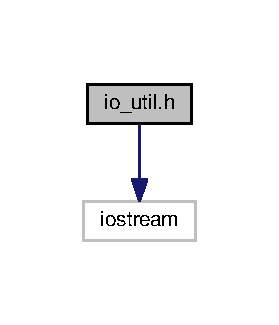
\includegraphics[width=134pt]{io__util_8h__incl}
\end{center}
\end{figure}
This graph shows which files directly or indirectly include this file\-:
\nopagebreak
\begin{figure}[H]
\begin{center}
\leavevmode
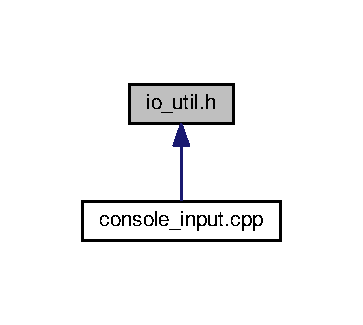
\includegraphics[width=309pt]{io__util_8h__dep__incl}
\end{center}
\end{figure}
\subsection*{Functions}
\begin{DoxyCompactItemize}
\item 
void \hyperlink{io__util_8h_ae8c346aa92fc891022a940f2c5c75f95}{setze\-\_\-schalter} (ios\-\_\-base\-::fmtflags format)
\item 
void \hyperlink{io__util_8h_acd3415eef442ced2b5e064f95f04b624}{swap} (int $\ast$x, int $\ast$y)
\end{DoxyCompactItemize}


\subsection{Function Documentation}
\hypertarget{io__util_8h_ae8c346aa92fc891022a940f2c5c75f95}{\index{io\-\_\-util.\-h@{io\-\_\-util.\-h}!setze\-\_\-schalter@{setze\-\_\-schalter}}
\index{setze\-\_\-schalter@{setze\-\_\-schalter}!io_util.h@{io\-\_\-util.\-h}}
\subsubsection[{setze\-\_\-schalter}]{\setlength{\rightskip}{0pt plus 5cm}void setze\-\_\-schalter (
\begin{DoxyParamCaption}
\item[{ios\-\_\-base\-::fmtflags}]{format}
\end{DoxyParamCaption}
)}}\label{io__util_8h_ae8c346aa92fc891022a940f2c5c75f95}
\hypertarget{io__util_8h_acd3415eef442ced2b5e064f95f04b624}{\index{io\-\_\-util.\-h@{io\-\_\-util.\-h}!swap@{swap}}
\index{swap@{swap}!io_util.h@{io\-\_\-util.\-h}}
\subsubsection[{swap}]{\setlength{\rightskip}{0pt plus 5cm}void swap (
\begin{DoxyParamCaption}
\item[{int $\ast$}]{x, }
\item[{int $\ast$}]{y}
\end{DoxyParamCaption}
)}}\label{io__util_8h_acd3415eef442ced2b5e064f95f04b624}

\hypertarget{pt__math__functions_8h}{\section{pt\-\_\-math\-\_\-functions.\-h File Reference}
\label{pt__math__functions_8h}\index{pt\-\_\-math\-\_\-functions.\-h@{pt\-\_\-math\-\_\-functions.\-h}}
}
{\ttfamily \#include $<$string$>$}\\*
Include dependency graph for pt\-\_\-math\-\_\-functions.\-h\-:\nopagebreak
\begin{figure}[H]
\begin{center}
\leavevmode
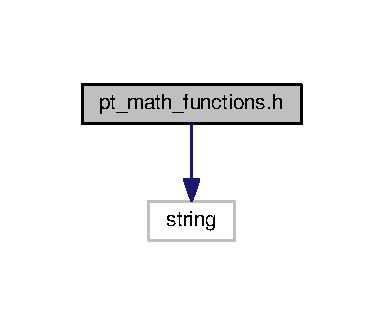
\includegraphics[width=184pt]{pt__math__functions_8h__incl}
\end{center}
\end{figure}
This graph shows which files directly or indirectly include this file\-:\nopagebreak
\begin{figure}[H]
\begin{center}
\leavevmode
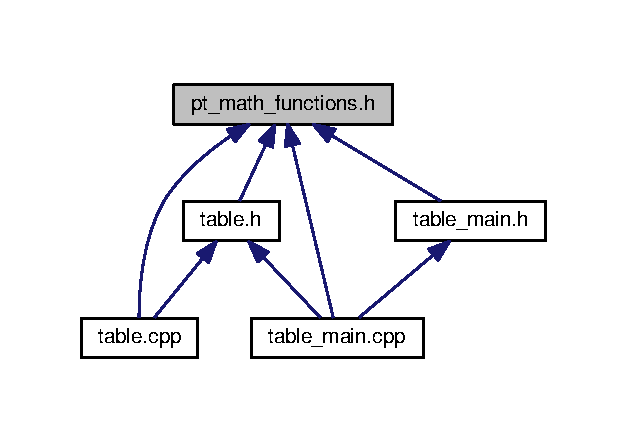
\includegraphics[width=302pt]{pt__math__functions_8h__dep__incl}
\end{center}
\end{figure}
\subsection*{Typedefs}
\begin{DoxyCompactItemize}
\item 
typedef double($\ast$ \hyperlink{pt__math__functions_8h_aaead49151b753b4ef6a4c84ee8aa8c36}{pt\-Math\-Function\-One} )(double)
\item 
typedef double($\ast$ \hyperlink{pt__math__functions_8h_ad6f1c83ac0e2e8b6e0393aeddfda805f}{pt\-Math\-Function\-Two} )(double, double)
\end{DoxyCompactItemize}


\subsection{Typedef Documentation}
\hypertarget{pt__math__functions_8h_aaead49151b753b4ef6a4c84ee8aa8c36}{\index{pt\-\_\-math\-\_\-functions.\-h@{pt\-\_\-math\-\_\-functions.\-h}!pt\-Math\-Function\-One@{pt\-Math\-Function\-One}}
\index{pt\-Math\-Function\-One@{pt\-Math\-Function\-One}!pt_math_functions.h@{pt\-\_\-math\-\_\-functions.\-h}}
\subsubsection[{pt\-Math\-Function\-One}]{\setlength{\rightskip}{0pt plus 5cm}typedef double($\ast$ pt\-Math\-Function\-One)(double)}}\label{pt__math__functions_8h_aaead49151b753b4ef6a4c84ee8aa8c36}
\hypertarget{pt__math__functions_8h_ad6f1c83ac0e2e8b6e0393aeddfda805f}{\index{pt\-\_\-math\-\_\-functions.\-h@{pt\-\_\-math\-\_\-functions.\-h}!pt\-Math\-Function\-Two@{pt\-Math\-Function\-Two}}
\index{pt\-Math\-Function\-Two@{pt\-Math\-Function\-Two}!pt_math_functions.h@{pt\-\_\-math\-\_\-functions.\-h}}
\subsubsection[{pt\-Math\-Function\-Two}]{\setlength{\rightskip}{0pt plus 5cm}typedef double($\ast$ pt\-Math\-Function\-Two)(double, double)}}\label{pt__math__functions_8h_ad6f1c83ac0e2e8b6e0393aeddfda805f}

\hypertarget{table_8cpp}{\section{table.\-cpp File Reference}
\label{table_8cpp}\index{table.\-cpp@{table.\-cpp}}
}
{\ttfamily \#include $<$iostream$>$}\\*
{\ttfamily \#include $<$sstream$>$}\\*
{\ttfamily \#include $<$cmath$>$}\\*
{\ttfamily \#include $<$climits$>$}\\*
{\ttfamily \#include $<$string$>$}\\*
{\ttfamily \#include $<$iomanip$>$}\\*
{\ttfamily \#include \char`\"{}console\-\_\-input.\-h\char`\"{}}\\*
{\ttfamily \#include \char`\"{}table.\-h\char`\"{}}\\*
{\ttfamily \#include \char`\"{}pt\-\_\-math\-\_\-functions.\-h\char`\"{}}\\*
Include dependency graph for table.\-cpp\-:
\nopagebreak
\begin{figure}[H]
\begin{center}
\leavevmode
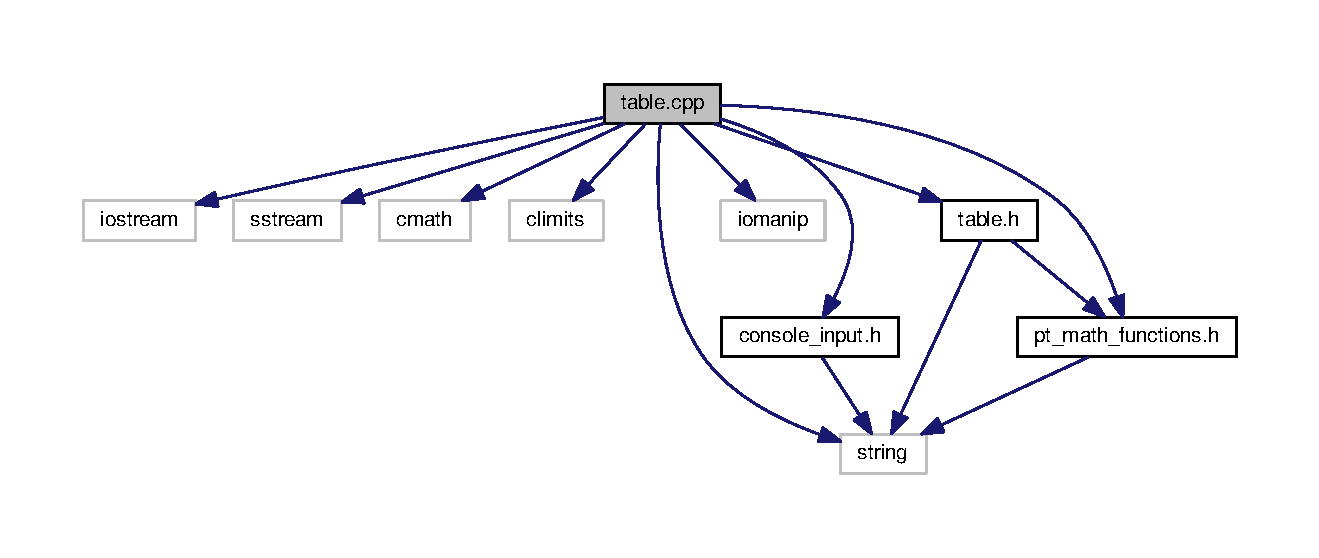
\includegraphics[width=350pt]{table_8cpp__incl}
\end{center}
\end{figure}
\subsection*{Functions}
\begin{DoxyCompactItemize}
\item 
string \hyperlink{table_8cpp_a27258c1b46c178213606bf2c13eb085b}{generate\-\_\-table} (\hyperlink{pt__math__functions_8h_aaead49151b753b4ef6a4c84ee8aa8c36}{pt\-Math\-Function\-One} function, string name, double start, double end, double steps, double row\-\_\-steps, int precision)
\item 
string \hyperlink{table_8cpp_abcc4aab1943a9c00c117c35b5c2e373f}{generate\-\_\-table} (\hyperlink{pt__math__functions_8h_ad6f1c83ac0e2e8b6e0393aeddfda805f}{pt\-Math\-Function\-Two} function, string name, double start, double end, double steps, double row\-\_\-steps, int precision, double param\-\_\-two)
\item 
string \hyperlink{table_8cpp_a1e9cb801bd8f49deb54fb1afc97cbdde}{generate\-\_\-table} (\hyperlink{pt__math__functions_8h_aaead49151b753b4ef6a4c84ee8aa8c36}{pt\-Math\-Function\-One} function, string name)
\item 
string \hyperlink{table_8cpp_a00e1177592ae74a7e1df38e1e1cd88f3}{generate\-\_\-table} (\hyperlink{pt__math__functions_8h_ad6f1c83ac0e2e8b6e0393aeddfda805f}{pt\-Math\-Function\-Two} function, string name)
\end{DoxyCompactItemize}


\subsection{Function Documentation}
\hypertarget{table_8cpp_a27258c1b46c178213606bf2c13eb085b}{\index{table.\-cpp@{table.\-cpp}!generate\-\_\-table@{generate\-\_\-table}}
\index{generate\-\_\-table@{generate\-\_\-table}!table.cpp@{table.\-cpp}}
\subsubsection[{generate\-\_\-table}]{\setlength{\rightskip}{0pt plus 5cm}string generate\-\_\-table (
\begin{DoxyParamCaption}
\item[{{\bf pt\-Math\-Function\-One}}]{function, }
\item[{string}]{name, }
\item[{double}]{start, }
\item[{double}]{end, }
\item[{double}]{steps, }
\item[{double}]{row\-\_\-steps, }
\item[{int}]{precision}
\end{DoxyParamCaption}
)}}\label{table_8cpp_a27258c1b46c178213606bf2c13eb085b}
Generates a value-\/table of a given function. The parameter of the given function is iterated by 'steps' and lies between the 'start' and 'end' value over the whole table.


\begin{DoxyParams}{Parameters}
{\em function} & Pointer to the function to generate values. \\
\hline
{\em name} & Name of the function. \\
\hline
{\em start} & Start value of the first parameter. \\
\hline
{\em end} & End value of the first parameter. \\
\hline
{\em steps} & Iteration stepts for the values between start, end. \\
\hline
{\em row\-\_\-steps} & Iteration steps for the columns of the table. \\
\hline
{\em precision} & Precision of the calculated values.\\
\hline
\end{DoxyParams}
\begin{DoxyReturn}{Returns}
a formatted value-\/table as a string. 
\end{DoxyReturn}
\hypertarget{table_8cpp_abcc4aab1943a9c00c117c35b5c2e373f}{\index{table.\-cpp@{table.\-cpp}!generate\-\_\-table@{generate\-\_\-table}}
\index{generate\-\_\-table@{generate\-\_\-table}!table.cpp@{table.\-cpp}}
\subsubsection[{generate\-\_\-table}]{\setlength{\rightskip}{0pt plus 5cm}string generate\-\_\-table (
\begin{DoxyParamCaption}
\item[{{\bf pt\-Math\-Function\-Two}}]{function, }
\item[{string}]{name, }
\item[{double}]{start, }
\item[{double}]{end, }
\item[{double}]{steps, }
\item[{double}]{row\-\_\-steps, }
\item[{int}]{precision, }
\item[{double}]{param\-\_\-two}
\end{DoxyParamCaption}
)}}\label{table_8cpp_abcc4aab1943a9c00c117c35b5c2e373f}
Generates a value-\/table of a given function. The first parameter of the given function is iterated by 'steps' and lies between the 'start' and 'end' value over the whole table. The second parameter 'param\-\_\-two' is static.


\begin{DoxyParams}{Parameters}
{\em function} & Pointer to the function to generate values. \\
\hline
{\em name} & Name of the function. \\
\hline
{\em start} & Start value of the first parameter. \\
\hline
{\em end} & End value of the first parameter. \\
\hline
{\em steps} & Iteration stepts for the values between start, end. \\
\hline
{\em row\-\_\-steps} & Iteration steps for the columns of the table. \\
\hline
{\em precision} & Precision of the calculated values. \\
\hline
{\em param\-\_\-two} & Second parameter for the function.\\
\hline
\end{DoxyParams}
\begin{DoxyReturn}{Returns}
a formatted value-\/table as a string. 
\end{DoxyReturn}
\hypertarget{table_8cpp_a1e9cb801bd8f49deb54fb1afc97cbdde}{\index{table.\-cpp@{table.\-cpp}!generate\-\_\-table@{generate\-\_\-table}}
\index{generate\-\_\-table@{generate\-\_\-table}!table.cpp@{table.\-cpp}}
\subsubsection[{generate\-\_\-table}]{\setlength{\rightskip}{0pt plus 5cm}string generate\-\_\-table (
\begin{DoxyParamCaption}
\item[{{\bf pt\-Math\-Function\-One}}]{function, }
\item[{string}]{name}
\end{DoxyParamCaption}
)}}\label{table_8cpp_a1e9cb801bd8f49deb54fb1afc97cbdde}
Promts the user to enter all values to generate the value-\/table for a given function. It then generates the value-\/table according the entered data.


\begin{DoxyParams}{Parameters}
{\em function} & Pointer to the function to generate values. \\
\hline
{\em name} & Name of the function.\\
\hline
\end{DoxyParams}
\begin{DoxyReturn}{Returns}
a formatted value-\/table as a string. 
\end{DoxyReturn}


Here is the call graph for this function\-:\nopagebreak
\begin{figure}[H]
\begin{center}
\leavevmode
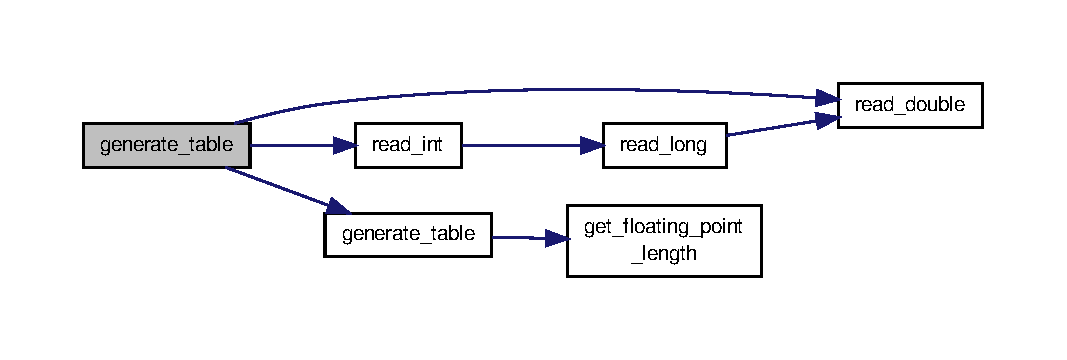
\includegraphics[width=350pt]{table_8cpp_a1e9cb801bd8f49deb54fb1afc97cbdde_cgraph}
\end{center}
\end{figure}


\hypertarget{table_8cpp_a00e1177592ae74a7e1df38e1e1cd88f3}{\index{table.\-cpp@{table.\-cpp}!generate\-\_\-table@{generate\-\_\-table}}
\index{generate\-\_\-table@{generate\-\_\-table}!table.cpp@{table.\-cpp}}
\subsubsection[{generate\-\_\-table}]{\setlength{\rightskip}{0pt plus 5cm}string generate\-\_\-table (
\begin{DoxyParamCaption}
\item[{{\bf pt\-Math\-Function\-Two}}]{function, }
\item[{string}]{name}
\end{DoxyParamCaption}
)}}\label{table_8cpp_a00e1177592ae74a7e1df38e1e1cd88f3}
Promts the user to enter all values to generate the value-\/table for a given function. It then generates the value-\/table according the entered data.


\begin{DoxyParams}{Parameters}
{\em function} & Pointer to the function to generate values. \\
\hline
{\em name} & Name of the function.\\
\hline
\end{DoxyParams}
\begin{DoxyReturn}{Returns}
a formatted value-\/table as a string. 
\end{DoxyReturn}


Here is the call graph for this function\-:\nopagebreak
\begin{figure}[H]
\begin{center}
\leavevmode
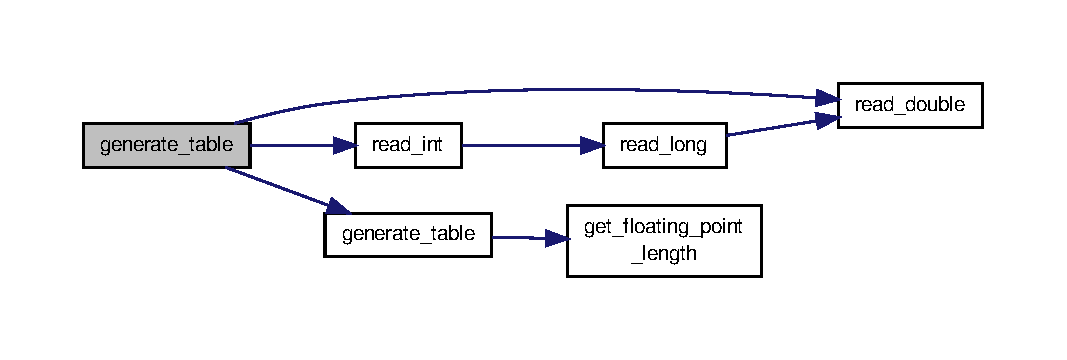
\includegraphics[width=350pt]{table_8cpp_a00e1177592ae74a7e1df38e1e1cd88f3_cgraph}
\end{center}
\end{figure}



\hypertarget{table_8h}{\section{table.\-h File Reference}
\label{table_8h}\index{table.\-h@{table.\-h}}
}
{\ttfamily \#include $<$string$>$}\\*
{\ttfamily \#include \char`\"{}pt\-\_\-math\-\_\-functions.\-h\char`\"{}}\\*
Include dependency graph for table.\-h\-:\nopagebreak
\begin{figure}[H]
\begin{center}
\leavevmode
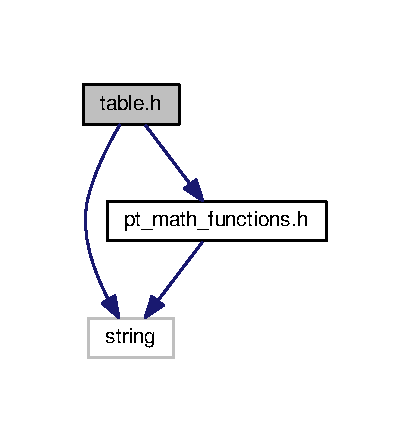
\includegraphics[width=196pt]{table_8h__incl}
\end{center}
\end{figure}
This graph shows which files directly or indirectly include this file\-:\nopagebreak
\begin{figure}[H]
\begin{center}
\leavevmode
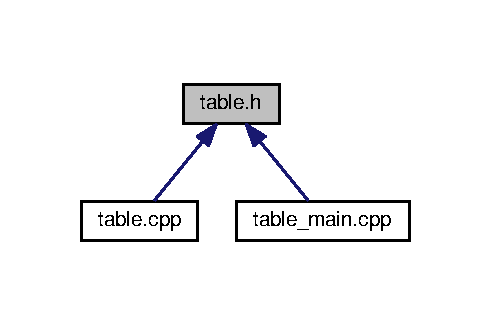
\includegraphics[width=236pt]{table_8h__dep__incl}
\end{center}
\end{figure}
\subsection*{Functions}
\begin{DoxyCompactItemize}
\item 
string \hyperlink{table_8h_abcc4aab1943a9c00c117c35b5c2e373f}{generate\-\_\-table} (\hyperlink{pt__math__functions_8h_ad6f1c83ac0e2e8b6e0393aeddfda805f}{pt\-Math\-Function\-Two} function, string name, double start, double end, double steps, double row\-\_\-steps, int precision, double param\-\_\-two)
\item 
string \hyperlink{table_8h_a27258c1b46c178213606bf2c13eb085b}{generate\-\_\-table} (\hyperlink{pt__math__functions_8h_aaead49151b753b4ef6a4c84ee8aa8c36}{pt\-Math\-Function\-One} function, string name, double start, double end, double steps, double row\-\_\-steps, int precision)
\item 
string \hyperlink{table_8h_a1e9cb801bd8f49deb54fb1afc97cbdde}{generate\-\_\-table} (\hyperlink{pt__math__functions_8h_aaead49151b753b4ef6a4c84ee8aa8c36}{pt\-Math\-Function\-One} function, string name)
\item 
string \hyperlink{table_8h_a00e1177592ae74a7e1df38e1e1cd88f3}{generate\-\_\-table} (\hyperlink{pt__math__functions_8h_ad6f1c83ac0e2e8b6e0393aeddfda805f}{pt\-Math\-Function\-Two} function, string name)
\item 
int \hyperlink{table_8h_a17774c1a04ac3735b8843f0d6b1f1afb}{get\-\_\-floating\-\_\-point\-\_\-length} (double number)
\end{DoxyCompactItemize}


\subsection{Function Documentation}
\hypertarget{table_8h_abcc4aab1943a9c00c117c35b5c2e373f}{\index{table.\-h@{table.\-h}!generate\-\_\-table@{generate\-\_\-table}}
\index{generate\-\_\-table@{generate\-\_\-table}!table.h@{table.\-h}}
\subsubsection[{generate\-\_\-table}]{\setlength{\rightskip}{0pt plus 5cm}string generate\-\_\-table (
\begin{DoxyParamCaption}
\item[{{\bf pt\-Math\-Function\-Two}}]{function, }
\item[{string}]{name, }
\item[{double}]{start, }
\item[{double}]{end, }
\item[{double}]{steps, }
\item[{double}]{row\-\_\-steps, }
\item[{int}]{precision, }
\item[{double}]{param\-\_\-two}
\end{DoxyParamCaption}
)}}\label{table_8h_abcc4aab1943a9c00c117c35b5c2e373f}
Generates a value-\/table of a given function. The first parameter of the given function is iterated by 'steps' and lies between the 'start' and 'end' value over the whole table. The second parameter 'param\-\_\-two' is static.


\begin{DoxyParams}{Parameters}
{\em function} & Pointer to the function to generate values. \\
\hline
{\em name} & Name of the function. \\
\hline
{\em start} & Start value of the first parameter. \\
\hline
{\em end} & End value of the first parameter. \\
\hline
{\em steps} & Iteration stepts for the values between start, end. \\
\hline
{\em row\-\_\-steps} & Iteration steps for the columns of the table. \\
\hline
{\em precision} & Precision of the calculated values. \\
\hline
{\em param\-\_\-two} & Second parameter for the function.\\
\hline
\end{DoxyParams}
\begin{DoxyReturn}{Returns}
a formatted value-\/table as a string. 
\end{DoxyReturn}
\hypertarget{table_8h_a27258c1b46c178213606bf2c13eb085b}{\index{table.\-h@{table.\-h}!generate\-\_\-table@{generate\-\_\-table}}
\index{generate\-\_\-table@{generate\-\_\-table}!table.h@{table.\-h}}
\subsubsection[{generate\-\_\-table}]{\setlength{\rightskip}{0pt plus 5cm}string generate\-\_\-table (
\begin{DoxyParamCaption}
\item[{{\bf pt\-Math\-Function\-One}}]{function, }
\item[{string}]{name, }
\item[{double}]{start, }
\item[{double}]{end, }
\item[{double}]{steps, }
\item[{double}]{row\-\_\-steps, }
\item[{int}]{precision}
\end{DoxyParamCaption}
)}}\label{table_8h_a27258c1b46c178213606bf2c13eb085b}
Generates a value-\/table of a given function. The parameter of the given function is iterated by 'steps' and lies between the 'start' and 'end' value over the whole table.


\begin{DoxyParams}{Parameters}
{\em function} & Pointer to the function to generate values. \\
\hline
{\em name} & Name of the function. \\
\hline
{\em start} & Start value of the first parameter. \\
\hline
{\em end} & End value of the first parameter. \\
\hline
{\em steps} & Iteration stepts for the values between start, end. \\
\hline
{\em row\-\_\-steps} & Iteration steps for the columns of the table. \\
\hline
{\em precision} & Precision of the calculated values.\\
\hline
\end{DoxyParams}
\begin{DoxyReturn}{Returns}
a formatted value-\/table as a string. 
\end{DoxyReturn}


Here is the call graph for this function\-:\nopagebreak
\begin{figure}[H]
\begin{center}
\leavevmode
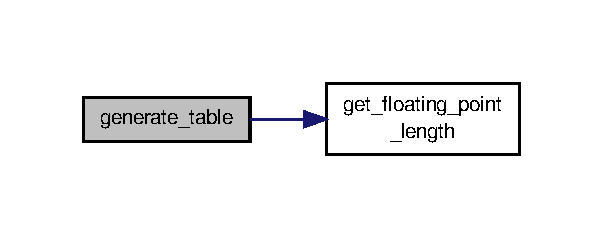
\includegraphics[width=290pt]{table_8h_a27258c1b46c178213606bf2c13eb085b_cgraph}
\end{center}
\end{figure}


\hypertarget{table_8h_a1e9cb801bd8f49deb54fb1afc97cbdde}{\index{table.\-h@{table.\-h}!generate\-\_\-table@{generate\-\_\-table}}
\index{generate\-\_\-table@{generate\-\_\-table}!table.h@{table.\-h}}
\subsubsection[{generate\-\_\-table}]{\setlength{\rightskip}{0pt plus 5cm}string generate\-\_\-table (
\begin{DoxyParamCaption}
\item[{{\bf pt\-Math\-Function\-One}}]{function, }
\item[{string}]{name}
\end{DoxyParamCaption}
)}}\label{table_8h_a1e9cb801bd8f49deb54fb1afc97cbdde}
Promts the user to enter all values to generate the value-\/table for a given function. It then generates the value-\/table according the entered data.


\begin{DoxyParams}{Parameters}
{\em function} & Pointer to the function to generate values. \\
\hline
{\em name} & Name of the function.\\
\hline
\end{DoxyParams}
\begin{DoxyReturn}{Returns}
a formatted value-\/table as a string. 
\end{DoxyReturn}


Here is the call graph for this function\-:\nopagebreak
\begin{figure}[H]
\begin{center}
\leavevmode
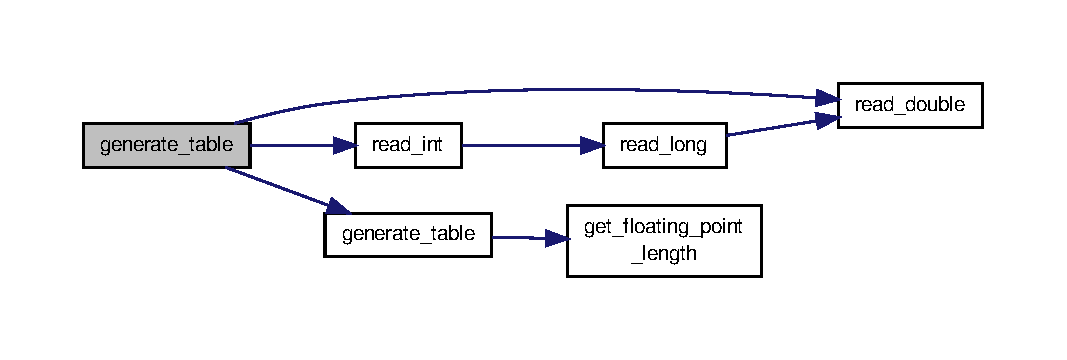
\includegraphics[width=350pt]{table_8h_a1e9cb801bd8f49deb54fb1afc97cbdde_cgraph}
\end{center}
\end{figure}


\hypertarget{table_8h_a00e1177592ae74a7e1df38e1e1cd88f3}{\index{table.\-h@{table.\-h}!generate\-\_\-table@{generate\-\_\-table}}
\index{generate\-\_\-table@{generate\-\_\-table}!table.h@{table.\-h}}
\subsubsection[{generate\-\_\-table}]{\setlength{\rightskip}{0pt plus 5cm}string generate\-\_\-table (
\begin{DoxyParamCaption}
\item[{{\bf pt\-Math\-Function\-Two}}]{function, }
\item[{string}]{name}
\end{DoxyParamCaption}
)}}\label{table_8h_a00e1177592ae74a7e1df38e1e1cd88f3}
Promts the user to enter all values to generate the value-\/table for a given function. It then generates the value-\/table according the entered data.


\begin{DoxyParams}{Parameters}
{\em function} & Pointer to the function to generate values. \\
\hline
{\em name} & Name of the function.\\
\hline
\end{DoxyParams}
\begin{DoxyReturn}{Returns}
a formatted value-\/table as a string. 
\end{DoxyReturn}


Here is the call graph for this function\-:\nopagebreak
\begin{figure}[H]
\begin{center}
\leavevmode
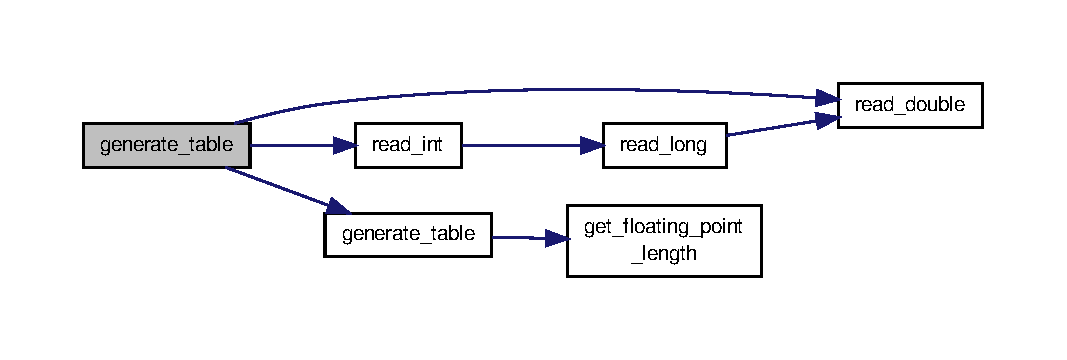
\includegraphics[width=350pt]{table_8h_a00e1177592ae74a7e1df38e1e1cd88f3_cgraph}
\end{center}
\end{figure}


\hypertarget{table_8h_a17774c1a04ac3735b8843f0d6b1f1afb}{\index{table.\-h@{table.\-h}!get\-\_\-floating\-\_\-point\-\_\-length@{get\-\_\-floating\-\_\-point\-\_\-length}}
\index{get\-\_\-floating\-\_\-point\-\_\-length@{get\-\_\-floating\-\_\-point\-\_\-length}!table.h@{table.\-h}}
\subsubsection[{get\-\_\-floating\-\_\-point\-\_\-length}]{\setlength{\rightskip}{0pt plus 5cm}int get\-\_\-floating\-\_\-point\-\_\-length (
\begin{DoxyParamCaption}
\item[{double}]{number}
\end{DoxyParamCaption}
)}}\label{table_8h_a17774c1a04ac3735b8843f0d6b1f1afb}
Gives back the length of a given floating point number.


\begin{DoxyParams}{Parameters}
{\em number} & Floating-\/point number to calculate the length.\\
\hline
\end{DoxyParams}
\begin{DoxyReturn}{Returns}
amouth of numerics including the point of the number. 
\end{DoxyReturn}

\hypertarget{table__main_8cpp}{\section{table\-\_\-main.\-cpp File Reference}
\label{table__main_8cpp}\index{table\-\_\-main.\-cpp@{table\-\_\-main.\-cpp}}
}
{\ttfamily \#include $<$iostream$>$}\\*
{\ttfamily \#include $<$cmath$>$}\\*
{\ttfamily \#include $<$string$>$}\\*
{\ttfamily \#include $<$cstdlib$>$}\\*
{\ttfamily \#include $<$iomanip$>$}\\*
{\ttfamily \#include \char`\"{}console\-\_\-input.\-h\char`\"{}}\\*
{\ttfamily \#include \char`\"{}table.\-h\char`\"{}}\\*
{\ttfamily \#include \char`\"{}pt\-\_\-math\-\_\-functions.\-h\char`\"{}}\\*
{\ttfamily \#include \char`\"{}table\-\_\-main.\-h\char`\"{}}\\*
{\ttfamily \#include \char`\"{}file\-\_\-controller.\-h\char`\"{}}\\*
Include dependency graph for table\-\_\-main.\-cpp\-:\nopagebreak
\begin{figure}[H]
\begin{center}
\leavevmode
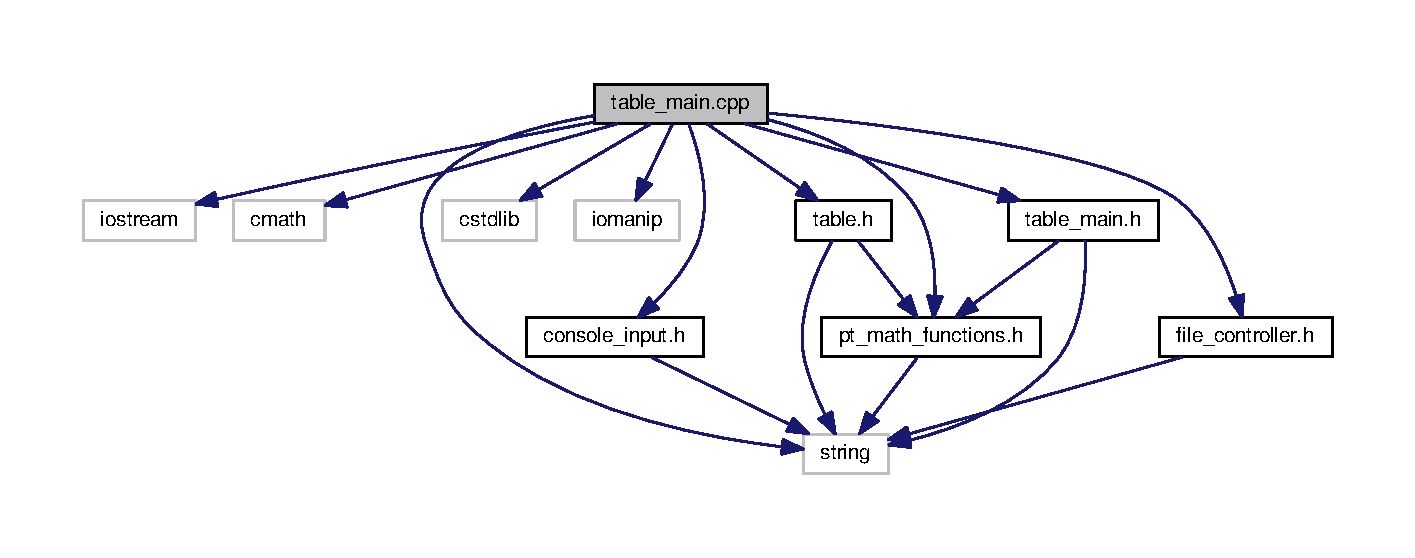
\includegraphics[width=350pt]{table__main_8cpp__incl}
\end{center}
\end{figure}
\subsection*{Functions}
\begin{DoxyCompactItemize}
\item 
int \hyperlink{table__main_8cpp_a0ddf1224851353fc92bfbff6f499fa97}{main} (int argc, char $\ast$argv\mbox{[}$\,$\mbox{]})
\item 
void \hyperlink{table__main_8cpp_a13a516479df3fbac2dec79ce076c160d}{handle\-\_\-action} (char $\ast$argv\mbox{[}$\,$\mbox{]})
\item 
void \hyperlink{table__main_8cpp_a352bcc46c3693e405cc701ece70bd196}{handle\-\_\-action} (int action)
\item 
void \hyperlink{table__main_8cpp_ad115f1168104746bd6f125391fbd0a99}{print\-\_\-actions} ()
\item 
int \hyperlink{table__main_8cpp_abd3bb699ef19768316dc170511fb0786}{get\-\_\-array\-\_\-index} (string item, const string items\mbox{[}$\,$\mbox{]}, int length)
\item 
string \hyperlink{table__main_8cpp_a9f56c4605d18aa78fcd4634bd55a0f87}{get\-\_\-function\-\_\-type} (string name)
\item 
bool \hyperlink{table__main_8cpp_a0bf5ec7e48000c167f6d7b5aeda3e4c4}{validate\-\_\-input} (int argc, char $\ast$argv\mbox{[}$\,$\mbox{]})
\item 
bool \hyperlink{table__main_8cpp_a4b45b9f42125840c08d7b70c1fd921bc}{validate\-\_\-param\-\_\-types} (string function\-\_\-type, char $\ast$argv\mbox{[}$\,$\mbox{]})
\item 
bool \hyperlink{table__main_8cpp_a040a1047545278bd502f2b1ec1b70759}{validate\-\_\-params\-\_\-length} (string function\-\_\-type, int argc)
\item 
bool \hyperlink{table__main_8cpp_aed78c4c2efe4694f7e61f0440294e674}{validate\-\_\-function\-\_\-name} (string name)
\end{DoxyCompactItemize}


\subsection{Function Documentation}
\hypertarget{table__main_8cpp_abd3bb699ef19768316dc170511fb0786}{\index{table\-\_\-main.\-cpp@{table\-\_\-main.\-cpp}!get\-\_\-array\-\_\-index@{get\-\_\-array\-\_\-index}}
\index{get\-\_\-array\-\_\-index@{get\-\_\-array\-\_\-index}!table_main.cpp@{table\-\_\-main.\-cpp}}
\subsubsection[{get\-\_\-array\-\_\-index}]{\setlength{\rightskip}{0pt plus 5cm}int get\-\_\-array\-\_\-index (
\begin{DoxyParamCaption}
\item[{string}]{item, }
\item[{const string}]{items\mbox{[}$\,$\mbox{]}, }
\item[{int}]{length}
\end{DoxyParamCaption}
)}}\label{table__main_8cpp_abd3bb699ef19768316dc170511fb0786}
Returns the index of a string inside an array of strings.


\begin{DoxyParams}{Parameters}
{\em item} & String to be searched in the array. \\
\hline
{\em items} & Array which contains the item.\\
\hline
\end{DoxyParams}
\begin{DoxyReturn}{Returns}
int index of the item in the array. -\/1 if not in the array. 
\end{DoxyReturn}
\hypertarget{table__main_8cpp_a9f56c4605d18aa78fcd4634bd55a0f87}{\index{table\-\_\-main.\-cpp@{table\-\_\-main.\-cpp}!get\-\_\-function\-\_\-type@{get\-\_\-function\-\_\-type}}
\index{get\-\_\-function\-\_\-type@{get\-\_\-function\-\_\-type}!table_main.cpp@{table\-\_\-main.\-cpp}}
\subsubsection[{get\-\_\-function\-\_\-type}]{\setlength{\rightskip}{0pt plus 5cm}string get\-\_\-function\-\_\-type (
\begin{DoxyParamCaption}
\item[{string}]{name}
\end{DoxyParamCaption}
)}}\label{table__main_8cpp_a9f56c4605d18aa78fcd4634bd55a0f87}
Returns a string representing the type of a function by its name. There are two defined types (\char`\"{}\-O\-N\-E\char`\"{} and \char`\"{}\-T\-W\-O\char`\"{}).


\begin{DoxyParams}{Parameters}
{\em name} & Name of the function to be checked.\\
\hline
\end{DoxyParams}
\begin{DoxyReturn}{Returns}
String O\-N\-E pt\-Math\-Function\-One\-: double ($\ast$)(double) T\-W\-O pt\-Math\-Function\-Two\-: double ($\ast$)(double, double) 
\end{DoxyReturn}
\hypertarget{table__main_8cpp_a13a516479df3fbac2dec79ce076c160d}{\index{table\-\_\-main.\-cpp@{table\-\_\-main.\-cpp}!handle\-\_\-action@{handle\-\_\-action}}
\index{handle\-\_\-action@{handle\-\_\-action}!table_main.cpp@{table\-\_\-main.\-cpp}}
\subsubsection[{handle\-\_\-action}]{\setlength{\rightskip}{0pt plus 5cm}void handle\-\_\-action (
\begin{DoxyParamCaption}
\item[{char $\ast$}]{argv\mbox{[}$\,$\mbox{]}}
\end{DoxyParamCaption}
)}}\label{table__main_8cpp_a13a516479df3fbac2dec79ce076c160d}
Handles a given action according the arguments array. Generates the table for the action and writes the table to a file. When the file already exists. The user gets prompted to chose if the file gets overwridden or not.


\begin{DoxyParams}{Parameters}
{\em $\ast$argv\mbox{[}$\,$\mbox{]}} & Arguments array from the program execution. \\
\hline
\end{DoxyParams}


Here is the call graph for this function\-:\nopagebreak
\begin{figure}[H]
\begin{center}
\leavevmode
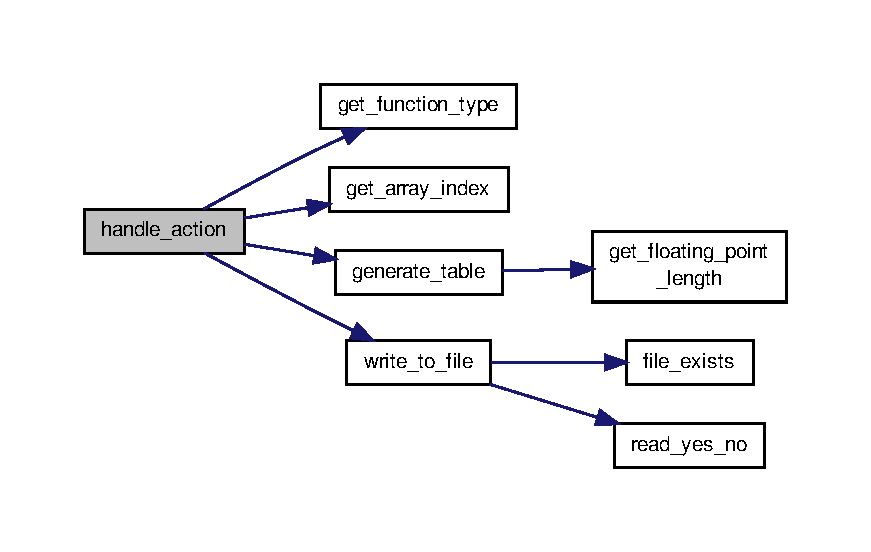
\includegraphics[width=350pt]{table__main_8cpp_a13a516479df3fbac2dec79ce076c160d_cgraph}
\end{center}
\end{figure}


\hypertarget{table__main_8cpp_a352bcc46c3693e405cc701ece70bd196}{\index{table\-\_\-main.\-cpp@{table\-\_\-main.\-cpp}!handle\-\_\-action@{handle\-\_\-action}}
\index{handle\-\_\-action@{handle\-\_\-action}!table_main.cpp@{table\-\_\-main.\-cpp}}
\subsubsection[{handle\-\_\-action}]{\setlength{\rightskip}{0pt plus 5cm}void handle\-\_\-action (
\begin{DoxyParamCaption}
\item[{int}]{action}
\end{DoxyParamCaption}
)}}\label{table__main_8cpp_a352bcc46c3693e405cc701ece70bd196}
Generates the table for e certain action given by the id. prints the table to the console and writes the table in a file chosen by the users input. If the file already exists, it promts the user to chose wheather to override it or to abord.


\begin{DoxyParams}{Parameters}
{\em action} & The action for witch to generate the table. \\
\hline
\end{DoxyParams}


Here is the call graph for this function\-:\nopagebreak
\begin{figure}[H]
\begin{center}
\leavevmode
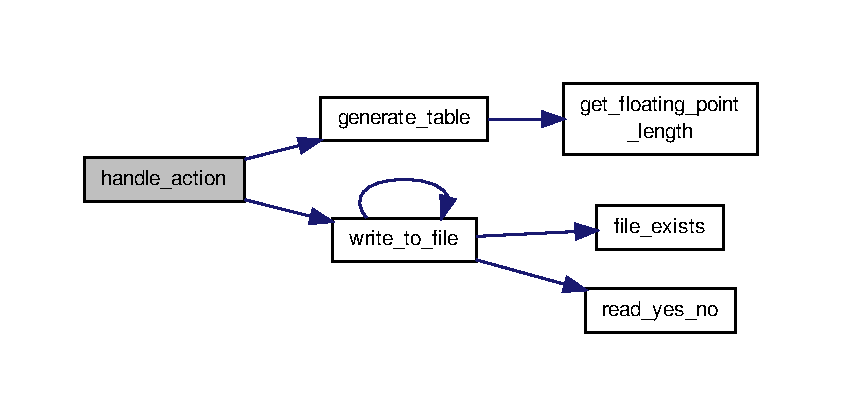
\includegraphics[width=350pt]{table__main_8cpp_a352bcc46c3693e405cc701ece70bd196_cgraph}
\end{center}
\end{figure}


\hypertarget{table__main_8cpp_a0ddf1224851353fc92bfbff6f499fa97}{\index{table\-\_\-main.\-cpp@{table\-\_\-main.\-cpp}!main@{main}}
\index{main@{main}!table_main.cpp@{table\-\_\-main.\-cpp}}
\subsubsection[{main}]{\setlength{\rightskip}{0pt plus 5cm}int main (
\begin{DoxyParamCaption}
\item[{int}]{argc, }
\item[{char $\ast$}]{argv\mbox{[}$\,$\mbox{]}}
\end{DoxyParamCaption}
)}}\label{table__main_8cpp_a0ddf1224851353fc92bfbff6f499fa97}
Entrypoint to the program 'tabelle'. Tabelle is a program to generate value-\/tables for the mathematical functions cos, sin, tan, acos, asin, atan, exp, log, log10, sqrt and pow.

The user can define following arguments\-:
\begin{DoxyEnumerate}
\item Name of the function
\item Start value of the table
\item End value of the table
\item Value for the iteration steps
\item Value for the steps of the rows (after how many iterations (colums) should start a new row)
\item Precision of the function output.
\item Additional parameter for the function (just for the function pow)
\item Filename of the file to save the table.
\end{DoxyEnumerate}

When a function needs additional parameters, the user has to enter these too. e.\-g. sin(x) =$>$ x is for all values between the start value and end value with the iteration of the step value. pow(x, exp) =$>$ exp has to be entered too. The iteration is just for x.


\begin{DoxyParams}{Parameters}
{\em argc} & Length of the arguments array. \\
\hline
{\em $\ast$argv\mbox{[}$\,$\mbox{]}} & Arguments array form the program execution. \\
\hline
\end{DoxyParams}


Here is the call graph for this function\-:\nopagebreak
\begin{figure}[H]
\begin{center}
\leavevmode
\includegraphics[width=350pt]{table__main_8cpp_a0ddf1224851353fc92bfbff6f499fa97_cgraph}
\end{center}
\end{figure}


\hypertarget{table__main_8cpp_ad115f1168104746bd6f125391fbd0a99}{\index{table\-\_\-main.\-cpp@{table\-\_\-main.\-cpp}!print\-\_\-actions@{print\-\_\-actions}}
\index{print\-\_\-actions@{print\-\_\-actions}!table_main.cpp@{table\-\_\-main.\-cpp}}
\subsubsection[{print\-\_\-actions}]{\setlength{\rightskip}{0pt plus 5cm}void print\-\_\-actions (
\begin{DoxyParamCaption}
{}
\end{DoxyParamCaption}
)}}\label{table__main_8cpp_ad115f1168104746bd6f125391fbd0a99}
Prints a description of the available actions to the console. \hypertarget{table__main_8cpp_aed78c4c2efe4694f7e61f0440294e674}{\index{table\-\_\-main.\-cpp@{table\-\_\-main.\-cpp}!validate\-\_\-function\-\_\-name@{validate\-\_\-function\-\_\-name}}
\index{validate\-\_\-function\-\_\-name@{validate\-\_\-function\-\_\-name}!table_main.cpp@{table\-\_\-main.\-cpp}}
\subsubsection[{validate\-\_\-function\-\_\-name}]{\setlength{\rightskip}{0pt plus 5cm}bool validate\-\_\-function\-\_\-name (
\begin{DoxyParamCaption}
\item[{string}]{name}
\end{DoxyParamCaption}
)}}\label{table__main_8cpp_aed78c4c2efe4694f7e61f0440294e674}
Checks if a function (by its name) is defined.


\begin{DoxyParams}{Parameters}
{\em name} & Name of the function to be checked.\\
\hline
\end{DoxyParams}
\begin{DoxyReturn}{Returns}
true if the function exists. fales if the function don't exists. 
\end{DoxyReturn}
\hypertarget{table__main_8cpp_a0bf5ec7e48000c167f6d7b5aeda3e4c4}{\index{table\-\_\-main.\-cpp@{table\-\_\-main.\-cpp}!validate\-\_\-input@{validate\-\_\-input}}
\index{validate\-\_\-input@{validate\-\_\-input}!table_main.cpp@{table\-\_\-main.\-cpp}}
\subsubsection[{validate\-\_\-input}]{\setlength{\rightskip}{0pt plus 5cm}bool validate\-\_\-input (
\begin{DoxyParamCaption}
\item[{int}]{argc, }
\item[{char $\ast$}]{argv\mbox{[}$\,$\mbox{]}}
\end{DoxyParamCaption}
)}}\label{table__main_8cpp_a0bf5ec7e48000c167f6d7b5aeda3e4c4}
Validates the input arguments. Checks if the function is available. Checks if there are enough argumends for the given function type. Checks if the arguments are in the right types.


\begin{DoxyParams}{Parameters}
{\em argc} & Lenght of the argument array. \\
\hline
{\em $\ast$argv\mbox{[}$\,$\mbox{]}} & Argument array.\\
\hline
\end{DoxyParams}
\begin{DoxyReturn}{Returns}
true when the arguments are valid. false when the arguments are invalid. 
\end{DoxyReturn}


Here is the call graph for this function\-:\nopagebreak
\begin{figure}[H]
\begin{center}
\leavevmode
\includegraphics[width=314pt]{table__main_8cpp_a0bf5ec7e48000c167f6d7b5aeda3e4c4_cgraph}
\end{center}
\end{figure}


\hypertarget{table__main_8cpp_a4b45b9f42125840c08d7b70c1fd921bc}{\index{table\-\_\-main.\-cpp@{table\-\_\-main.\-cpp}!validate\-\_\-param\-\_\-types@{validate\-\_\-param\-\_\-types}}
\index{validate\-\_\-param\-\_\-types@{validate\-\_\-param\-\_\-types}!table_main.cpp@{table\-\_\-main.\-cpp}}
\subsubsection[{validate\-\_\-param\-\_\-types}]{\setlength{\rightskip}{0pt plus 5cm}bool validate\-\_\-param\-\_\-types (
\begin{DoxyParamCaption}
\item[{string}]{function\-\_\-type, }
\item[{char $\ast$}]{argv\mbox{[}$\,$\mbox{]}}
\end{DoxyParamCaption}
)}}\label{table__main_8cpp_a4b45b9f42125840c08d7b70c1fd921bc}
Validates the type of the arguments according the type of the given function to be called.


\begin{DoxyParams}{Parameters}
{\em function\-\_\-type} & Type of the function (\char`\"{}\-O\-N\-E\char`\"{} ore \char`\"{}\-T\-W\-O\char`\"{}) \\
\hline
{\em $\ast$argv\mbox{[}$\,$\mbox{]}} & Input arguments.\\
\hline
\end{DoxyParams}
\begin{DoxyReturn}{Returns}
true when the argument types fit the functions type. false when the argument types don't fit the functions type. 
\end{DoxyReturn}
\hypertarget{table__main_8cpp_a040a1047545278bd502f2b1ec1b70759}{\index{table\-\_\-main.\-cpp@{table\-\_\-main.\-cpp}!validate\-\_\-params\-\_\-length@{validate\-\_\-params\-\_\-length}}
\index{validate\-\_\-params\-\_\-length@{validate\-\_\-params\-\_\-length}!table_main.cpp@{table\-\_\-main.\-cpp}}
\subsubsection[{validate\-\_\-params\-\_\-length}]{\setlength{\rightskip}{0pt plus 5cm}bool validate\-\_\-params\-\_\-length (
\begin{DoxyParamCaption}
\item[{string}]{function\-\_\-type, }
\item[{int}]{argc}
\end{DoxyParamCaption}
)}}\label{table__main_8cpp_a040a1047545278bd502f2b1ec1b70759}
Validates the argument length according a given function type.


\begin{DoxyParams}{Parameters}
{\em function\-\_\-type} & Type of the function (\char`\"{}\-O\-N\-E\char`\"{} ore \char`\"{}\-T\-W\-O\char`\"{}) \\
\hline
{\em argc} & Length of the argument array.\\
\hline
\end{DoxyParams}
\begin{DoxyReturn}{Returns}
true if the argument length fit the function type false if the argument length don fit the function type. 
\end{DoxyReturn}

\hypertarget{table__main_8h}{\section{table\-\_\-main.\-h File Reference}
\label{table__main_8h}\index{table\-\_\-main.\-h@{table\-\_\-main.\-h}}
}
{\ttfamily \#include $<$string$>$}\\*
{\ttfamily \#include \char`\"{}pt\-\_\-math\-\_\-functions.\-h\char`\"{}}\\*
Include dependency graph for table\-\_\-main.\-h\-:\nopagebreak
\begin{figure}[H]
\begin{center}
\leavevmode
\includegraphics[width=209pt]{table__main_8h__incl}
\end{center}
\end{figure}
This graph shows which files directly or indirectly include this file\-:\nopagebreak
\begin{figure}[H]
\begin{center}
\leavevmode
\includegraphics[width=162pt]{table__main_8h__dep__incl}
\end{center}
\end{figure}
\subsection*{Functions}
\begin{DoxyCompactItemize}
\item 
int \hyperlink{table__main_8h_a0ddf1224851353fc92bfbff6f499fa97}{main} (int argc, char $\ast$argv\mbox{[}$\,$\mbox{]})
\item 
void \hyperlink{table__main_8h_ad115f1168104746bd6f125391fbd0a99}{print\-\_\-actions} ()
\item 
void \hyperlink{table__main_8h_a352bcc46c3693e405cc701ece70bd196}{handle\-\_\-action} (int action)
\item 
void \hyperlink{table__main_8h_a13a516479df3fbac2dec79ce076c160d}{handle\-\_\-action} (char $\ast$argv\mbox{[}$\,$\mbox{]})
\item 
bool \hyperlink{table__main_8h_a0bf5ec7e48000c167f6d7b5aeda3e4c4}{validate\-\_\-input} (int argc, char $\ast$argv\mbox{[}$\,$\mbox{]})
\item 
bool \hyperlink{table__main_8h_a0f86595eb8dcc1bb533ed3ee87a5c603}{validate\-\_\-function\-\_\-name} (string function\-\_\-name)
\item 
bool \hyperlink{table__main_8h_acfb44a8598d2bdc702d3ba190e156231}{validate\-\_\-start\-\_\-end\-\_\-range} (double start, double end)
\item 
bool \hyperlink{table__main_8h_a036e051985dce76f757d19f2dfb78800}{validate\-\_\-steps\-\_\-range} (double step, double row\-\_\-step)
\item 
bool \hyperlink{table__main_8h_a040a1047545278bd502f2b1ec1b70759}{validate\-\_\-params\-\_\-length} (string function\-\_\-type, int argc)
\item 
bool \hyperlink{table__main_8h_a4b45b9f42125840c08d7b70c1fd921bc}{validate\-\_\-param\-\_\-types} (string function\-\_\-type, char $\ast$argv\mbox{[}$\,$\mbox{]})
\item 
int \hyperlink{table__main_8h_a0bb0944ea7a4f2b01d571239acf8cce9}{get\-\_\-array\-\_\-index} (string name, const string names\mbox{[}$\,$\mbox{]}, int length)
\item 
string \hyperlink{table__main_8h_a9f56c4605d18aa78fcd4634bd55a0f87}{get\-\_\-function\-\_\-type} (string name)
\end{DoxyCompactItemize}


\subsection{Function Documentation}
\hypertarget{table__main_8h_a0bb0944ea7a4f2b01d571239acf8cce9}{\index{table\-\_\-main.\-h@{table\-\_\-main.\-h}!get\-\_\-array\-\_\-index@{get\-\_\-array\-\_\-index}}
\index{get\-\_\-array\-\_\-index@{get\-\_\-array\-\_\-index}!table_main.h@{table\-\_\-main.\-h}}
\subsubsection[{get\-\_\-array\-\_\-index}]{\setlength{\rightskip}{0pt plus 5cm}int get\-\_\-array\-\_\-index (
\begin{DoxyParamCaption}
\item[{string}]{item, }
\item[{const string}]{items\mbox{[}$\,$\mbox{]}, }
\item[{int}]{length}
\end{DoxyParamCaption}
)}}\label{table__main_8h_a0bb0944ea7a4f2b01d571239acf8cce9}
Returns the index of a string inside an array of strings.


\begin{DoxyParams}{Parameters}
{\em item} & String to be searched in the array. \\
\hline
{\em items} & Array which contains the item.\\
\hline
\end{DoxyParams}
\begin{DoxyReturn}{Returns}
int index of the item in the array. -\/1 if not in the array. 
\end{DoxyReturn}
\hypertarget{table__main_8h_a9f56c4605d18aa78fcd4634bd55a0f87}{\index{table\-\_\-main.\-h@{table\-\_\-main.\-h}!get\-\_\-function\-\_\-type@{get\-\_\-function\-\_\-type}}
\index{get\-\_\-function\-\_\-type@{get\-\_\-function\-\_\-type}!table_main.h@{table\-\_\-main.\-h}}
\subsubsection[{get\-\_\-function\-\_\-type}]{\setlength{\rightskip}{0pt plus 5cm}string get\-\_\-function\-\_\-type (
\begin{DoxyParamCaption}
\item[{string}]{name}
\end{DoxyParamCaption}
)}}\label{table__main_8h_a9f56c4605d18aa78fcd4634bd55a0f87}
Returns a string representing the type of a function by its name. There are two defined types (\char`\"{}\-O\-N\-E\char`\"{} and \char`\"{}\-T\-W\-O\char`\"{}).


\begin{DoxyParams}{Parameters}
{\em name} & Name of the function to be checked.\\
\hline
\end{DoxyParams}
\begin{DoxyReturn}{Returns}
String O\-N\-E pt\-Math\-Function\-One\-: double ($\ast$)(double) T\-W\-O pt\-Math\-Function\-Two\-: double ($\ast$)(double, double) 
\end{DoxyReturn}
\hypertarget{table__main_8h_a352bcc46c3693e405cc701ece70bd196}{\index{table\-\_\-main.\-h@{table\-\_\-main.\-h}!handle\-\_\-action@{handle\-\_\-action}}
\index{handle\-\_\-action@{handle\-\_\-action}!table_main.h@{table\-\_\-main.\-h}}
\subsubsection[{handle\-\_\-action}]{\setlength{\rightskip}{0pt plus 5cm}void handle\-\_\-action (
\begin{DoxyParamCaption}
\item[{int}]{action}
\end{DoxyParamCaption}
)}}\label{table__main_8h_a352bcc46c3693e405cc701ece70bd196}
Generates the table for e certain action given by the id. prints the table to the console and writes the table in a file chosen by the users input. If the file already exists, it promts the user to chose wheather to override it or to abord.


\begin{DoxyParams}{Parameters}
{\em action} & The action for witch to generate the table. \\
\hline
\end{DoxyParams}


Here is the call graph for this function\-:
\nopagebreak
\begin{figure}[H]
\begin{center}
\leavevmode
\includegraphics[width=350pt]{table__main_8h_a352bcc46c3693e405cc701ece70bd196_cgraph}
\end{center}
\end{figure}


\hypertarget{table__main_8h_a13a516479df3fbac2dec79ce076c160d}{\index{table\-\_\-main.\-h@{table\-\_\-main.\-h}!handle\-\_\-action@{handle\-\_\-action}}
\index{handle\-\_\-action@{handle\-\_\-action}!table_main.h@{table\-\_\-main.\-h}}
\subsubsection[{handle\-\_\-action}]{\setlength{\rightskip}{0pt plus 5cm}void handle\-\_\-action (
\begin{DoxyParamCaption}
\item[{char $\ast$}]{argv\mbox{[}$\,$\mbox{]}}
\end{DoxyParamCaption}
)}}\label{table__main_8h_a13a516479df3fbac2dec79ce076c160d}
Handles a given action according the arguments array. Generates the table for the action and writes the table to a file. When the file already exists. The user gets prompted to chose if the file gets overwridden or not.


\begin{DoxyParams}{Parameters}
{\em $\ast$argv\mbox{[}$\,$\mbox{]}} & Arguments array from the program execution. \\
\hline
\end{DoxyParams}


Here is the call graph for this function\-:
\nopagebreak
\begin{figure}[H]
\begin{center}
\leavevmode
\includegraphics[width=350pt]{table__main_8h_a13a516479df3fbac2dec79ce076c160d_cgraph}
\end{center}
\end{figure}


\hypertarget{table__main_8h_a0ddf1224851353fc92bfbff6f499fa97}{\index{table\-\_\-main.\-h@{table\-\_\-main.\-h}!main@{main}}
\index{main@{main}!table_main.h@{table\-\_\-main.\-h}}
\subsubsection[{main}]{\setlength{\rightskip}{0pt plus 5cm}int main (
\begin{DoxyParamCaption}
\item[{int}]{argc, }
\item[{char $\ast$}]{argv\mbox{[}$\,$\mbox{]}}
\end{DoxyParamCaption}
)}}\label{table__main_8h_a0ddf1224851353fc92bfbff6f499fa97}
Entrypoint to the program 'tabelle'. Tabelle is a program to generate value-\/tables for the mathematical functions cos, sin, tan, acos, asin, atan, exp, log, log10, sqrt and pow.

The user can define following arguments\-:
\begin{DoxyEnumerate}
\item Name of the function
\item Start value of the table
\item End value of the table
\item Value for the iteration steps
\item Value for the steps of the rows (after how many iterations (colums) should start a new row)
\item Precision of the function output.
\item Additional parameter for the function (just for the function pow)
\item Filename of the file to save the table.
\end{DoxyEnumerate}

When a function needs additional parameters, the user has to enter these too. e.\-g. sin(x) =$>$ x is for all values between the start value and end value with the iteration of the step value. pow(x, exp) =$>$ exp has to be entered too. The iteration is just for x.


\begin{DoxyParams}{Parameters}
{\em argc} & Length of the arguments array. \\
\hline
{\em $\ast$argv\mbox{[}$\,$\mbox{]}} & Arguments array form the program execution. \\
\hline
\end{DoxyParams}


Here is the call graph for this function\-:
\nopagebreak
\begin{figure}[H]
\begin{center}
\leavevmode
\includegraphics[width=350pt]{table__main_8h_a0ddf1224851353fc92bfbff6f499fa97_cgraph}
\end{center}
\end{figure}


\hypertarget{table__main_8h_ad115f1168104746bd6f125391fbd0a99}{\index{table\-\_\-main.\-h@{table\-\_\-main.\-h}!print\-\_\-actions@{print\-\_\-actions}}
\index{print\-\_\-actions@{print\-\_\-actions}!table_main.h@{table\-\_\-main.\-h}}
\subsubsection[{print\-\_\-actions}]{\setlength{\rightskip}{0pt plus 5cm}void print\-\_\-actions (
\begin{DoxyParamCaption}
{}
\end{DoxyParamCaption}
)}}\label{table__main_8h_ad115f1168104746bd6f125391fbd0a99}
Prints a description of the available actions to the console. \hypertarget{table__main_8h_a0f86595eb8dcc1bb533ed3ee87a5c603}{\index{table\-\_\-main.\-h@{table\-\_\-main.\-h}!validate\-\_\-function\-\_\-name@{validate\-\_\-function\-\_\-name}}
\index{validate\-\_\-function\-\_\-name@{validate\-\_\-function\-\_\-name}!table_main.h@{table\-\_\-main.\-h}}
\subsubsection[{validate\-\_\-function\-\_\-name}]{\setlength{\rightskip}{0pt plus 5cm}bool validate\-\_\-function\-\_\-name (
\begin{DoxyParamCaption}
\item[{string}]{name}
\end{DoxyParamCaption}
)}}\label{table__main_8h_a0f86595eb8dcc1bb533ed3ee87a5c603}
Checks if a function (by its name) is defined.


\begin{DoxyParams}{Parameters}
{\em name} & Name of the function to be checked.\\
\hline
\end{DoxyParams}
\begin{DoxyReturn}{Returns}
true if the function exists. fales if the function don't exists. 
\end{DoxyReturn}
\hypertarget{table__main_8h_a0bf5ec7e48000c167f6d7b5aeda3e4c4}{\index{table\-\_\-main.\-h@{table\-\_\-main.\-h}!validate\-\_\-input@{validate\-\_\-input}}
\index{validate\-\_\-input@{validate\-\_\-input}!table_main.h@{table\-\_\-main.\-h}}
\subsubsection[{validate\-\_\-input}]{\setlength{\rightskip}{0pt plus 5cm}bool validate\-\_\-input (
\begin{DoxyParamCaption}
\item[{int}]{argc, }
\item[{char $\ast$}]{argv\mbox{[}$\,$\mbox{]}}
\end{DoxyParamCaption}
)}}\label{table__main_8h_a0bf5ec7e48000c167f6d7b5aeda3e4c4}
Validates the input arguments. Checks if the function is available. Checks if there are enough argumends for the given function type. Checks if the arguments are in the right types.


\begin{DoxyParams}{Parameters}
{\em argc} & Lenght of the argument array. \\
\hline
{\em $\ast$argv\mbox{[}$\,$\mbox{]}} & Argument array.\\
\hline
\end{DoxyParams}
\begin{DoxyReturn}{Returns}
true when the arguments are valid. false when the arguments are invalid. 
\end{DoxyReturn}


Here is the call graph for this function\-:\nopagebreak
\begin{figure}[H]
\begin{center}
\leavevmode
\includegraphics[width=314pt]{table__main_8h_a0bf5ec7e48000c167f6d7b5aeda3e4c4_cgraph}
\end{center}
\end{figure}


\hypertarget{table__main_8h_a4b45b9f42125840c08d7b70c1fd921bc}{\index{table\-\_\-main.\-h@{table\-\_\-main.\-h}!validate\-\_\-param\-\_\-types@{validate\-\_\-param\-\_\-types}}
\index{validate\-\_\-param\-\_\-types@{validate\-\_\-param\-\_\-types}!table_main.h@{table\-\_\-main.\-h}}
\subsubsection[{validate\-\_\-param\-\_\-types}]{\setlength{\rightskip}{0pt plus 5cm}bool validate\-\_\-param\-\_\-types (
\begin{DoxyParamCaption}
\item[{string}]{function\-\_\-type, }
\item[{char $\ast$}]{argv\mbox{[}$\,$\mbox{]}}
\end{DoxyParamCaption}
)}}\label{table__main_8h_a4b45b9f42125840c08d7b70c1fd921bc}
Validates the type of the arguments according the type of the given function to be called.


\begin{DoxyParams}{Parameters}
{\em function\-\_\-type} & Type of the function (\char`\"{}\-O\-N\-E\char`\"{} ore \char`\"{}\-T\-W\-O\char`\"{}) \\
\hline
{\em $\ast$argv\mbox{[}$\,$\mbox{]}} & Input arguments.\\
\hline
\end{DoxyParams}
\begin{DoxyReturn}{Returns}
true when the argument types fit the functions type. false when the argument types don't fit the functions type. 
\end{DoxyReturn}
\hypertarget{table__main_8h_a040a1047545278bd502f2b1ec1b70759}{\index{table\-\_\-main.\-h@{table\-\_\-main.\-h}!validate\-\_\-params\-\_\-length@{validate\-\_\-params\-\_\-length}}
\index{validate\-\_\-params\-\_\-length@{validate\-\_\-params\-\_\-length}!table_main.h@{table\-\_\-main.\-h}}
\subsubsection[{validate\-\_\-params\-\_\-length}]{\setlength{\rightskip}{0pt plus 5cm}bool validate\-\_\-params\-\_\-length (
\begin{DoxyParamCaption}
\item[{string}]{function\-\_\-type, }
\item[{int}]{argc}
\end{DoxyParamCaption}
)}}\label{table__main_8h_a040a1047545278bd502f2b1ec1b70759}
Validates the argument length according a given function type.


\begin{DoxyParams}{Parameters}
{\em function\-\_\-type} & Type of the function (\char`\"{}\-O\-N\-E\char`\"{} ore \char`\"{}\-T\-W\-O\char`\"{}) \\
\hline
{\em argc} & Length of the argument array.\\
\hline
\end{DoxyParams}
\begin{DoxyReturn}{Returns}
true if the argument length fit the function type false if the argument length don fit the function type. 
\end{DoxyReturn}
\hypertarget{table__main_8h_acfb44a8598d2bdc702d3ba190e156231}{\index{table\-\_\-main.\-h@{table\-\_\-main.\-h}!validate\-\_\-start\-\_\-end\-\_\-range@{validate\-\_\-start\-\_\-end\-\_\-range}}
\index{validate\-\_\-start\-\_\-end\-\_\-range@{validate\-\_\-start\-\_\-end\-\_\-range}!table_main.h@{table\-\_\-main.\-h}}
\subsubsection[{validate\-\_\-start\-\_\-end\-\_\-range}]{\setlength{\rightskip}{0pt plus 5cm}bool validate\-\_\-start\-\_\-end\-\_\-range (
\begin{DoxyParamCaption}
\item[{double}]{start, }
\item[{double}]{end}
\end{DoxyParamCaption}
)}}\label{table__main_8h_acfb44a8598d2bdc702d3ba190e156231}
\hypertarget{table__main_8h_a036e051985dce76f757d19f2dfb78800}{\index{table\-\_\-main.\-h@{table\-\_\-main.\-h}!validate\-\_\-steps\-\_\-range@{validate\-\_\-steps\-\_\-range}}
\index{validate\-\_\-steps\-\_\-range@{validate\-\_\-steps\-\_\-range}!table_main.h@{table\-\_\-main.\-h}}
\subsubsection[{validate\-\_\-steps\-\_\-range}]{\setlength{\rightskip}{0pt plus 5cm}bool validate\-\_\-steps\-\_\-range (
\begin{DoxyParamCaption}
\item[{double}]{step, }
\item[{double}]{row\-\_\-step}
\end{DoxyParamCaption}
)}}\label{table__main_8h_a036e051985dce76f757d19f2dfb78800}

%--- End generated contents ---

% Index
\newpage
\phantomsection
\addcontentsline{toc}{chapter}{Index}
\printindex

\end{document}
